\documentclass[10pt,sigconf]{acmart}

\usepackage{booktabs}
\usepackage{algorithmic}
\usepackage{algorithm}
\usepackage{hyperref, url}
\usepackage{pdfpages}

\usepackage{amsfonts}
\newcommand{\Z}{\mathbb{Z}}

\setcopyright{none}
\settopmatter{printacmref=false,authorsperrow=2}
\renewcommand\footnotetextcopyrightpermission[1]{} 
%\pagestyle{plain}
\pagenumbering{gobble}

\graphicspath{{images/}}

% verbatim grey start
\usepackage{fancyvrb,newverbs,xcolor}
\definecolor{cverbbg}{gray}{0.95}
\newenvironment{cverbatim}
 {\SaveVerbatim{cverb}}
 {\endSaveVerbatim
  \flushleft\fboxrule=0pt\fboxsep=.5em
  \colorbox{cverbbg}{\BUseVerbatim{cverb}}%
  \endflushleft
}
\newenvironment{lcverbatim}
 {\SaveVerbatim{cverb}}
 {\endSaveVerbatim
  \flushleft\fboxrule=0pt\fboxsep=.5em
  \colorbox{cverbbg}{%
    \makebox[\dimexpr\linewidth-2\fboxsep][l]{\BUseVerbatim{cverb}}%
  }
  \endflushleft
}

\newcommand{\ctexttt}[1]{\colorbox{cverbbg}{\texttt{#1}}}
\newverbcommand{\cverb}
  {\setbox\verbbox\hbox\bgroup}
  {\egroup\colorbox{cverbbg}{\box\verbbox}}
% verbatim grey end



\begin{document}

\acmConference[COMP90043]{COMP90043 Cryptography and Security}{Semester 2, 2018}{Melbourne}

%%%

\noindent {\Huge Team Reflective Statement}
\vspace{1em}

\noindent \textbf{Yiru Pan (Vivian)}'s reflective statement:

In this research project, I am mainly in charge of Lamport digital signature scheme. The reason why I chose this scheme is this scheme can resist quantum computing, which sounds very intriguing. At the beginning, I need to search related academic papers, and uploaded them in google drive for other teammates to read and learn. Then I attended every group meeting, and shared my ideas with others proactively. In the experiment stage, I implemented code of Lamport scheme, and uploaded it to Spartan to test, finished all designed scenarios. During the implementation, I knew the reason why Lamport can resist quantum computing, while other schemes cannot. Lamport uses large number of hash function calculations instead of relying on algorithm complexity. Its security depends on the performance of hash function. The state of art implementation of Lamport is to use SHA256, which has been proved safe in most scenarios. My code can accomplish three steps, including key generation, signing message, signature verification. During the test, 
with the input scale increasing, the measurement data can demonstrate that the Lamport scheme is dominant by key generation, because it contains a large number of hash calculations in key generation stage.
 What is more, I finished design of presentation slides, and generated all data form in a uniform format. During the video making stage, I helped other teammates to truncate speech sheet and control time limit, I cooperated well with other teammates, and learned very useful skills from others, such as using Latex to edit report and using python to generate plot. These skills are very helpful for my future academic life.

From this research project, I also learned other digital signature schemes, which broaden my knowledge scope significantly. I learned how to write professional academic paper in Latex, and the professional evaluation metric for different schemes. This project is a good opportunity for me to sharpen my research skills as well as teamwork skills. We did a good job in the presentation, and improved in the final report per the comments from teacher and tutor. I indeed learned a lot from this subject, and this subject is one of my favorite subjects during my master life. Thanks for lecturer, tutors and my teammates, it has been a pleasure to learn this subject. 

%%% Vivian END
\vspace{1em}

\noindent \textbf{Tenglun Tan (Tan Tan)}'s reflective statement:

Initially I was very excited to do this research project, since last semester I have been working with a professor in the cryptography area, meeting with several "Blockchain Maniacs" and doing literature reviews on some recent research papers every week. In this project our team choose the Experiment track, which gives me a chance to apply the theory in practice. Our team works in a very cooperative and efficient way. As an active contributor to our team, I was in charge of the ECDSA part, learning ECDSA algorithms, running experiments, and analysing results that can be used to draw the conclusion in the overall comparison part. I wrote ECDSA part in the report and present it in our presentation. In the end I was surprised to find out that concepts such as point multiplication on elliptic curve that was very confusing to me several months ago become clearer now. When reflecting back, I found out it was the research papers I have read in this area and the experiments I have done that helps me understand the mechanism of ECDSA better. I analyzed twelve papers talking about ECDSA with high citations. Several of them illustrates the key generation, message signing and signature verification thoroughly so that I will not miss any point of the algorithms. I also learned how previous researchers did their performance and security experiments, so I can stand on the shoulders of giant to research further. My teammates gave a lot of help as well. We held several group meetings to share ideas and discuss the progress we have made for the past period. From them, I was exposed to the new algorithms such as EdDSA and Lamport, whose performance results are very exciting. At the beginning I used pure python package to implement ECDSA and found out it was pretty slow to generate key pairs, even slower than RSA. My teammate Victor helped me find out another implementation of ECDSA using C which is nearly 10 times faster than the pure python package. For the report and presentation, I used python matplotlib  to generate appropriate figures for all the plots and Vivian used Mac Numbers to generate appropriate tables. I also learned the truth that implementation method does matter for the same algorithms from my team working experience. In the overall comparison part, I contributed my insights and got a big picture of the object of this project. I really enjoyed this team learning and working experience.

%%% Tan END
\vspace{1em}

\noindent \textbf{Zhuohan Xie (Theo)}'s reflective statement:

In this project, we distributed our experiments into four digital algorithms, RSA, ECDSA, EdDSA and lamport and assigned each team member to explore one of these algorithms and conducted the cross-comparison after that. 
My part is EdDSA, which is a very new algorithm that is believed to achieve higher security with higher speed. Since it is not covered in the lecture materials, I have to read two papers which I cited in the EdDSA part to get an idea about what EdDSA is.
After that, I tried to implement this algorithm on OpenSSL, but it seems that it is not well supported by OpenSSL, I could generate key pairs by OpenSSL but could not sign the messages or verify the signatures with it. Therefore, I gave up OpenSSL and tried to find python package called ed25519.
After understanding the principles of this package, I imported this package in my python code to generate key pairs, sign the messages and verify the signatures and measure the time of each step. It works well on my local laptop and the time each step takes is small. However, An interesting thing is that I found this package did not work well when I uploaded it to the cloud server which is provided by my teammate. It took much longer time on the cloud server than on my local laptop. After that, I experimented two other packages, PyNacl and libNacl with assistance of my teammate. These two algorithms work well on the cloud server, and I compared the performance of these three and analysed the experiment results in the presentation slides and report. 
In the presentation, I made EdDSA part of slides and contributed my insights in the cross comparison and helped to build comparison metric in the last slide and explained EdDSA part in the recording video. My slide is mainly focused on the experiment I did in EdDSA since it is the main focus of our research topic.

As for report, I wrote the EdDSA section, it is not just about the experiment part like I mentioned above in the slide, it is the whole thing about EdDSA, a general overview of this algorithm, parameters of this algorithm, mathematical equations behind message signing and signature verification processes. I read several papers so as to get the gist and write this part. Also, I illustrated my experiment results in detail in performance part, which is also covered in the slide, but with more analysis. 
Finally, the other main part of EdDSA section of the report is the security part, in this part, I not only analysed what security level EdDSA could provide, but also found a valid attack against it and wrote the detail in the report to illustrate that even though EdDSA might defend side channel attacks, but it could still be valuable to fault attacks and came to a conclusion that protections or countermeasures against fault attacks should be considered if the algorithm is applied in areas where they are possible.
Overall, I enjoyed our team work and learned significant knowledge from this project.

%%% Theo END
\vspace{1em}

\noindent \textbf{San Kho Lin (Victor)}'s reflective statement:

For the algorithm, I choose RSA since I wanted to study deeper and go-beyond the topic taught in the class. The motivation is related to my real life working experience where I need to develop and deploy distributed systems and oversee many Cloud Computing Clusters and instances. On daily basis, tools such as SSH, OpenSSL, PyCA and BouncyCastle are my tool-of-trade to develop and deploy software in client-server environment. Generating SSL certificates, revoking and maintaining certificates, signing software releases, as such daily routines involve dealing with Public Key Cryptography and, encounter with RSA is inevitable. I am glad I have enrolled this subject and undertake rigorous assessments to strengthen my knowledge further on cryptography and underlying mathematics.

In term of contribution to team work, my teammates are kind enough to nominate me as a team leader. As a team leader, I initiated to carry out research methods, gather related quality literature, brainstorm benchmarking methodology, formulate evaluation strategy, propose tools and quality implementations, write Python code, setup Cloud VM, perform cross comparison runtime and analysis, draw conclusion, take care of report format and overall editorial on Latex. Furthermore, I also try my best to understand and extend my contribution on the rest of the digital signature algorithms presenting in this research paper. Closely collaboration with my teammate make me reach to the deeper level of understanding on the presenting topics; of which doing it all by myself alone might not be possible within short amount of time. As a team, it is our mutual goal to get highest mark on the research work we present. Therefore, all team members work hard to present the quality research and excellent experiment at our best effort. All in all, I believe, we are the high performance team!

\vspace{2em}

\noindent For Latex authoring, we use Overleaf (\url{https://www.overleaf.com}). For report format, we use ACM conference paper and citation format in 10pt, two-columns template.
\begin{itemize}
    \item \url{https://www.acm.org/publications/proceedings-template}
    \item \url{https://github.com/borisveytsman/acmart/}
\end{itemize}

\vspace{2em}

\noindent Team 73 \\
yirup, tenglunt, zhuohanx, sanl1 \\
Research Project: Experiment Track \\
Digital Signature Schemes Evaluation \\
COMP90043 Cryptography and Security, 2018 SM2

\newpage


% Reflective Statement End


\title{Digital Signature Schemes Evaluation}
%\subtitle{COMP90043: Cryptography and Security}


\author{San Kho Lin}
\affiliation{\institution{829463}\city{University of Melbourne}}
\email{sanl1@student.unimelb.edu.au}

\author{Yiru Pan}
\affiliation{\institution{889832}\city{University of Melbourne}}
\email{yirup@student.unimelb.edu.au}

\author{Tenglun Tan}
\affiliation{\institution{876792}\city{University of Melbourne}}
\email{tenglunt@student.unimelb.edu.au}

\author{Zhuohan Xie}
\affiliation{\institution{871089}\city{University of Melbourne}}
\email{zhuohanx@student.unimelb.edu.au}


% \begin{abstract}
% This paper provides a sample of a \LaTeX\ document which conforms, somewhat loosely, to the formatting guidelines for ACM SIG Proceedings.\footnote{This is an abstract footnote}
% \end{abstract}
% \keywords{RSA, ECDSA, EdDSA, Lamport signature}

\maketitle

\section{Introduction}

Digital signature is a mathematical scheme that used to validate the authenticity of a message. By signing a digital document, one can ensure that the signer is the original author of the digital document and, other parties cannot modify it. It is widely used technique to add authentication, integrity and non-repudiation properties to a digital document. The idea of digital signature is one of the applied public key cryptography originally discussed in Diffie-Hellman paper \cite{Diffie:2006:NDC:2263321.2269104}. %Several digital schemes have been proven to provide valid authentication for signing and verifying a message. 
Particularly, we are interested in 3 digital signature algorithms -- RSA, ECC and Lamport signature -- to evaluate and compare them.

\subsection{Background}

RSA \cite{Rivest:1978:MOD:359340.359342} is the well-known implementation of public key cryptography and digital signature scheme. It is based on the hard factorization problem of two large prime numbers $p$ and $q$ such that it is not computationally feasible for anyone to factor $n$ i.e. $n = p \cdot q$. We use RSA as our baseline for formulating evaluation metrics.

Elliptic Curve Cryptography (ECC) is another efficient public key cryptography technique. Particularly, we focus on ECDSA \cite{Kerry13fipspub} which is based on the difficulty of solving discrete logarithm problem in Elliptic Curve group. %-- also known as elliptic curve discrete logarithm problem. 
We also investigate EdDSA \cite{Bernstein2012} that has used twisted Edwards curves modifications and parameter tuning for top performance. ECC is well-known for providing greater security with smaller key sizes. %This feature is desirable for saving computation resources and bandwidth in securing mobile devices and sensor networks traffic. It is a trending digital signature scheme such as cryptocurrencies like Bitcoin have made use of it. 
However, ECC discrete logarithms computation is known to be broken by Shor's algorithm \cite{Shor:1997:PAP:264393.264406} on a hypothetical quantum computer.

Lamport one-time digital signature scheme \cite{lamport} is an efficient method for constructing a digital signature. %One time means that a signature can be used only once due to the algorithm design. When verifying the signature, it reveals a part of the private key. Lamport signatures can be built from any cryptographically secure one-way hash function. 
It has been increased interest due to characteristics such as fast verification, one-way property and quantum-proof. RSA, ECC rely on the computational hard problems which are prone to be broken when a quantum computer is practically implemented.

\subsection{Motivation}

In this project, we explore 3 digital signature schemes: RSA, ECC, and Lamport signature scheme. The main idea of choosing these 3 schemes is their uniqueness in technique and mathematical approaches. We study their mathematical foundations and associated process for key generation, signing and verification of digital signatures. We perform experiments to measure their performance such as timing private/public keys generation, signing and verifying the data messages. We also discuss their performance-security trade-offs, complexity and implementations. Our objective is to observe characteristic and performance of each scheme and, produce qualitative evaluation metrics and discuss suitable application domain for each of them.

\subsection{Experiment Setup and Tools}

%Since we focus on observing performance comparison and security trade-off evaluation, 
We begin our research on publicly accessible quality implementation of these algorithms. After experimenting many initial trials, we have empirically finalised to choose the following cryptographic tools and libraries for experiment.
\begin{itemize}
    \item OpenSSL (\url{https://www.openssl.org})
    \item NaCl (\url{https://nacl.cr.yp.to})
    \item LibSodium (\url{https://libsodium.org})
\end{itemize}

Our choice of programming language is Python and, therefore we have investigated tools and wrapper around these chosen libraries. We have also written our best effort implementation, sourced and utilised third party implementation for each digital signature scheme when we deem appropriate to strengthen our discussion and experiments. Such activity, sources and details are further cited and discussed in respective section.

Additionally, in order to get the uniform experiment result, we use NeCTAR (\url{https://nectar.org.au}) Research Cloud virtual machine (VM) instance for all our runtime benchmarking. This NeCTAR Cloud VM is the \textit{m2.medium} instance flavour which comprise of \textbf{2 vCPU} and \textbf{6GB RAM} memory. The choice of base operating system is \textit{Ubuntu 18.04.1 LTS}. We name this Cloud VM to \textbf{Krypton} for easy reference. 
% \begin{table}
% \caption{Chosen Cryptographic Implementations}
%     \begin{tabular}{ |p{2cm}|p{5.5cm}|  }
%     \hline
%     \textbf{Name} & \textbf{Link} \\
%     \hline
%     OpenSSL & \url{https://www.openssl.org} \\
%     \hline
%     NaCl & \url{https://nacl.cr.yp.to} \\
%     \hline
%     libsodium & \url{https://libsodium.org} \\
%     \hline    
%     \end{tabular}
%   \label{tab:libTable}
% \end{table}

\noindent For the test datasets, we use the Comma-separated Values (CSV) data that is publicly available at:
\begin{itemize}
    \item \href{http://eforexcel.com/wp/downloads-18-sample-csv-files-data-sets-for-testing-sales/}{http://eforexcel.com/wp/category/downloads/}
\end{itemize}

The average message size is 160 bytes per-line in plain text format. Initially, we also aim to experiment on different data formats (jpg, doc). Since our focus is observing algorithm characteristic, a small plain text message is sufficient enough for our experiment. Besides, we justify that the message will get hash function applied before signing process.

The remainder of the paper is organised as follows. Sections 2, 3, 4 and 5 covers RSA, ECDSA, EdDSA and Lamport signature scheme investigation details. Section 6 provides cross comparison performance analysis and quantitative research on generating runtime measurement. Finally, section 7 gives qualitative research outcome, concluding remarks and identify future works.

%%% RSA START

\section{RSA}

%According to Diffie-Hellman paper \cite{Diffie:2006:NDC:2263321.2269104}, the general public key cryptography exhibits one-way and trap-door function along with a pair of keys known as public key and private key. One-way function implies that there is no computationally feasible way to revert the process that had done. Trap-door function implies that only by knowing a particular component (therefore, a trap-door) such as decryption key or private key, it can be possible to revert the process; otherwise impossible. RSA \cite{Rivest:1978:MOD:359340.359342} is one of the Public Key Cryptography System (PKCS) that realise Diffie-Hellman's public key cryptography idea with Integer Modulo in Group $\Z^{*}_{N}$. 

RSA \cite{Rivest:1978:MOD:359340.359342} is well-studied and popular Public Key Cryptography System (PKCS) appear in many standards such as NIST \cite{Kerry13fipspub}, RFC8017 \cite{rfc8017}. It is based on two computationally hard problems known as Integer Factorisation problem (as one-way function) and RSA problem (as trap-door function). The factoring large integers is well-known "hard" problem in computational mathematics and Number theory. Especially in RSA, we consider two large prime numbers such that $N = p \cdot q$; by only knowing $N$, it is infeasible to find prime factors $p$ and $q$ of $N$. Thus, integer factoring problem serves as one-way function in RSA.

RSA propose working on Integer Modulo multiplicative Group $\Z^{*}_{N}$ such that let $e$, $d$ be two integers satisfying $e \cdot d = 1 \mod \varphi(N)$ where $\varphi(N) = (p - 1) \cdot (q - 1)$. Then, RSA defines $e$ be public exponent, $d$ be private exponent and $N$ be public modulus. Therefore, $\langle N, e \rangle$ pair forms public key; similarly $\langle N, d \rangle$ pair forms private key. For the integer representation of message $M \in \Z^{*}_{N}$, encryption defines as $C = M^e \mod N$ and, decryption defines as $M = C^d \mod N$ which indeed satisfy $M = (M^e)^{d} = C^d \pmod N$. Note that for given publicly known $N$ and $e$ for $C = M^e \mod N$, RSA make strong assumption that it is infeasible to determine $M$. It is the second computational "hard" problem that manifest in RSA. RSA states that finding $e$th root of modulo integer $N$ of unknown factorisation is hard and, conclude as RSA problem. Only if we know the private component $d$ then we can decrypt the message and, therefore, RSA problem serves as trap-door function.

For computing RSA digital signature, it is the inverted operation of encryption and decryption process. That is, signing operation is $S = M^d \mod N$ and, signature verification on $M$ is $S^e = M \mod N$. 

\subsection{Signature Security}

We observe that RSA problem is stronger assumption than Integer Factoring problem. It means that when it might be possible to find an efficient algorithm for the RSA problem but finding efficient algorithm for the factoring problem remains infeasible. According to \cite{case2003beginner}, we learn that the General Number Field Sieve (GNFS) algorithm is the best known efficient algorithm for integer factoring which has run time complexity of $exp\big((c + o(1)) n^{1/3} log^{2/3}n\big)$ on $n$-bit integers for some $c < 2$. Generally speaking, it is sub-exponential time complexity.

Since introduction of RSA and more than 30-years, RSA "hard" problem assumptions withstand mathematical attacks, when RSA is implemented and used properly. However, studies \cite{boneh1999twenty} \cite{coppersmith1997small} \cite{coron2000new} show that many attacks are still possible for improper use of RSA algorithm. In the context of research presenting in this paper, we are interested in attacks related to RSA digital signature scheme and, its countermeasures. In previous section, we explain mathematical foundation on how basis RSA work. This simple version of RSA is also referred to as \textbf{Textbook RSA} in cryptography literature. 

The textbook RSA version has some implication on multiplicative property of RSA signature which lead to \textbf{Existential Forgery attack} such that for some messages $M1$ and $M2$, it is $(M1 * M2)^d = M1^d * M2^d$; if $S1$ is signature of $M1$ and $S2$ is signature of $M2$; then, $(S1 * S2)$ is the signature of $(M1 * M2)$, therefore signature forgery is possible. Also, since signature is the inverse of encryption operation, what if the same key pair is used for signing and encryption. Furthermore, what if we try to sign very long message i.e. $M$ > modulo $N$.

Another attack to consider for RSA signature is \textbf{Blinding attack}. Suppose Bob wishes Alice to sign a message $M$ but Alice normally refuse to do. Alice public key is $\langle N, e \rangle$ then, Bob choose random $X \in \Z_{N}^*$ and, create a blinded message $M_b = X^e \cdot M \mod N$ and ask Alice to sign $M_b$. Since $M$ is hidden due to multiplicative process, Alice may sign $S_b = (M_{b})^d \mod N$. Now Bob can compute signature for $M$ as $S = S_b \cdot X^{-1} \mod N$. We can now show that: 
\begin{align*}
    S^e = (S_{b})^e / X^{e} = (M_b)^{ed} / X^{e} \equiv M_b / X^{e} = M \pmod N
\end{align*}
Hence, $S$ is the signature for $M$.

Another important aspect of RSA signature security is the Low Public Exponent $e$. According to RSA standard RFC8017 \cite{rfc8017}, it defines $e$ can be any random integers between $3 \leq e \leq (N - 1)$, as long as $e$ is relatively prime to public modulus $N$ i.e. $\gcd(e, N) = 1$. It may be desirable to choose lower $e$ value for performance purpose during exponentiation by repeated squaring and multiplying algorithm computation step of RSA process. However, \cite{boneh1999twenty} survey many attacks related to implication on choosing low public exponent value (e.g. $e=3$) such as Broadcast attack using Chinese Remainder theorem and, efficient Coppersmith's \cite{coppersmith1997small} theorem on finding small roots of polynomials modulo a composite $N$. By observation, we find that Fermat primes\footnote{\url{https://en.wikipedia.org/wiki/Fermat\_number}} ($F_n = 2^{2^n} + 1$), especially $F4 = 2^{16}+ 1 = 65537$ is recommended to defeat certain attacks. \cite{boneh1999twenty} explains that when $65537$ is used, signature verification just need 17 multiplications compare to approximately 1000 multiplications when a random $e \leq \varphi(N)$. This is due the fact that the binary representation of $65537$ number\footnote{\url{https://en.wikipedia.org/wiki/65,537}} contains most $0$s binary state, which effectively fast in low-level machine code computation.

Furthermore, we also investigate the public exponent $e$ value usage of well-known implementations. In OpenSSL, it generates $e$ with $F4$ option\footnote{\url{https://www.openssl.org/docs/manmaster/man1/genrsa.html}} by default and, also offers $e=3$. In OpenSSH (v5.3)\footnote{\url{https://github.com/openssh/openssh-portable/blob/V_5_3/key.c\#L688}}, it uses $e = 35$ and,  PuTTY\footnote{\url{https://git.tartarus.org/?p=simon/putty.git;a=blob;f=sshrsag.c;hb=HEAD\#l9}} uses $e = 37$.

Therefore, we can observe that RSA public exponent $e$ is empirical choice over some interesting \textit{Prime Number} that depends on standard practice and, a good compromise between performance and security trade-off.

\subsection{Padding and Hashing}

The real world RSA implementation has to consider technique to countermeasure the issue arise from the basic textbook RSA. \cite{boneh2000textbook} further explains that without proper pre-possessing scheme, the textbook RSA signing and encryption is fundamentally insecure. RSA standard PKCS\#1 introduces hash-then-sign padding scheme such that it calculates the cryptographic hash of the input message, together with some fixed padding, and this is then used as an input for the RSA function. However, such padding scheme is simple and strictly deterministic i.e. for the same input and key, the output will always be the same. In \cite{bleichenbacher1998chosen}, it explains how Chosen Ciphertext Attacks can be mounted against observing the returns query of decryption-box on only one bit telling whether the ciphertext correlates to some unknown block (i.e. padding block) of data encrypted using PKCS\#1, and the attacker could eventually gain information on $C^d$.

Therefore, later RSA standard improvement includes a more complex format schemes such as Optimal Asymmetric Encryption Padding (OAEP) \cite{bellare1994optimal} for encryption process and, Probabilistic Signature Scheme (PSS) \cite{bellare2001probabilistic} for signature process. \cite{bock2011rsa} survey and review the PSS scheme and how it works. It also explains the key concept such as Hash-then-Sign, Mask Generating Function (MGF) and Full Domain Hashing (FDH). In a nutshell, PSS adds randomness to the signature process, and a technique for reverting the randomness during verification. Randomisation is crucial to prevent dictionary attacks. This is important as attacks may be possible if the source of the random numbers is weak.

\subsection{Performance}

We use PyCA \cite{PyCACryptography} with OpenSSL backend for RSA experiment. To get RSA performance in reasonable secured setting, we setup parameters as follows:
\small{
\begin{lcverbatim}
public_exponent = 65537
param_hash = hashes.SHA256()
openssl_backend = default_backend()
rsa_padding = padding.PSS( \
    mgf=padding.MGF1(param_hash), \
    salt_length = padding.PSS.MAX_LENGTH)
\end{lcverbatim}
}

We, then vary the different key sizes ranging from bits value of 1024, 2048, 3072, 4096, 7680 and 15360 with a fixed load of signing only \textbf{one} message. The choice of key sizes are from NIST's 
Recommendation for Key Management \cite{nistKeysizes} standard; except 4096-bit is chosen empirically due to popular usage over Internet for digital certificate purpose. We fix the load to one message because we want to observe the highest 15360-bit runtime performance.

\begin{figure}
\centering
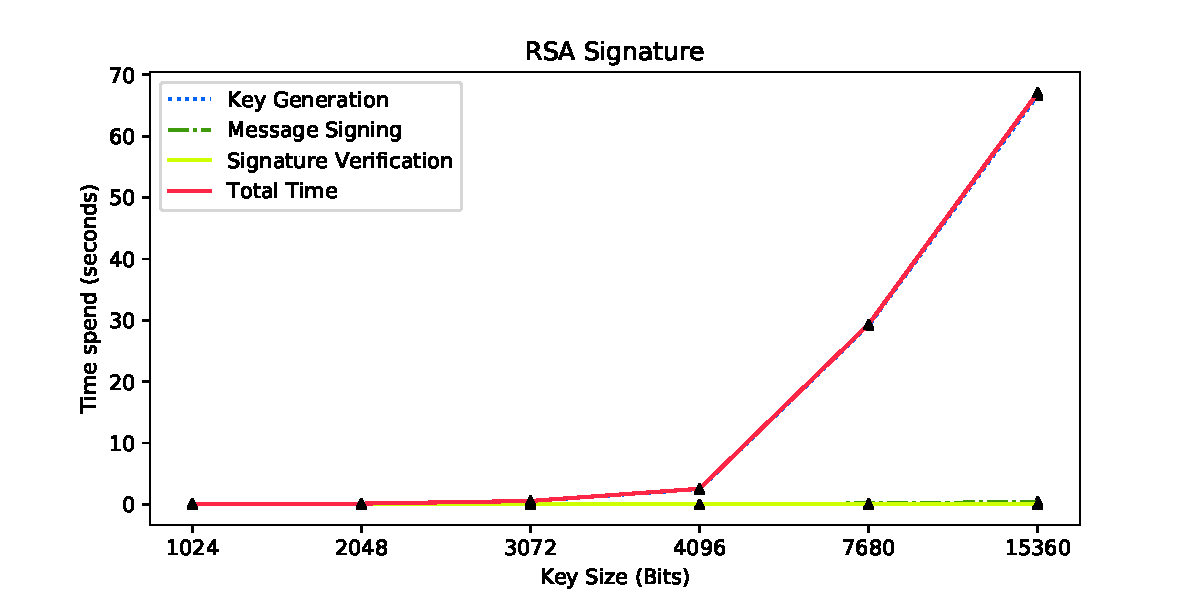
\includegraphics[scale=0.45]{RSA_Varying_Keysize_Runtime_Graph}
\caption{\small{RSA Varying Keysize Runtime}}
\label{fig:RSA_Varying_Keysize_Runtime_Graph}
\end{figure}

As depict in Figure~\ref{fig:RSA_Varying_Keysize_Runtime_Graph}, RSA key generation is predominantly influence the overall runtime. Message signing and signature verification runtime become insignificant and taken less than a second in all key sizes. Furthermore, as we can see in the graph, RSA key generation runtime is exponential growth rate as we increase key size from 4096-bit to 15360-bit. According to NIST \cite{nistKeysizes}, RSA key length 1024-bit and less should not use anymore. 2048-bit key size is acceptable usage until 2030. Key length of more than 3072-bit should use after 2030.

Even though it will not be linear, by hypothesis, we can approximate $N$ number of messages runtime for key size 15360-bit by just multiply 1 message runtime reported in graph. For example, 70s x 1000 messages = 70,000s time required for key size 15360-bit. We emphasize the notion of signing 1 message with highest key size 15360-bit as the baseline evaluation metric for comparing in later sections.

%In summary, all elementary attacks are possible when using the basic plain textbook RSA signature scheme. The fundamental of RSA algorithm is deterministic and the absence of random component in algorithm process makes it semantically insecure\footnote{\url{https://en.wikipedia.org/wiki/Semantic\_security}}. Generally, adversary can easily mount elementary attacks against plain textbook RSA method, even though underlying mathematical models are computationally "hard" problem to reverse.

%To counter such elementary attacks (language frequency analysis, dictionary attack) and other type of attacks \cite{boneh1999twenty}, RSA has to employ some random padding pre-processing scheme before signing or encryption process. We also discuss that simple padding scheme are still vulnerable to Adaptive Chosen Ciphertext attack and, therefore using complex padding scheme like PSS to make the signature cipher text indistinguishable for language analysis as well as effectively removing the multiplicative property of RSA algorithm. In practice, RSA algorithm needs to consider additional factors to be optimally secured and a better performed cryptosystem.

%%% RSA END



%%% ECDSA START

\section{ECDSA}

The Elliptic Curve Digital Signature Algorithm (ECDSA) realizes Digital Signature Algorithm (DSA) using the Elliptic Curve Cryptography (ECC). In 1999, ECDSA was accepted as an ANSI standard. In 2000, it was accepted as NIST and IEEE standards \cite{johnson2001elliptic}. Breaking traditional digital signature scheme such as RSA and DSA needs to solve integer factorization problem or discrete logarithm problem, where both of them only take sub-exponential time. Comparing to RSA and DSA, the running time to break ECDSA is fully exponential. Therefore, ECDSA can achieve same security with smaller key sizes and faster running time.

\subsection{ECDSA Algorithm}

Same as all the other digital signature schemes, ECDSA contains three algorithms representing three stages: Key Generation, Message Signing and Signature Verification. Computing Elliptic Curve Discrete Logarithm Problem (ECDLP) in the group of points on an elliptic curve defined over a finite field is the main difficulty that ensures the security of a public key system \cite{imem2015comparison}. Typically, we use SHA-256 as the hash function in Message Signing and Signature Verification stages.
\\
\\
\noindent \textbf{Domain Parameters:} \quad There are five domain parameters in ECDSA algorithms that are common to all entities participating in the network: $(q, E, G, n, h)$. These include a chosen elliptic curve $E$ defined over a finite field $F_q$ and a base point $GE \in E(F_q)$. The Parameters table below further illustrates the meaning of each parameter.
\\
\\
\noindent Parameters of ECDSA:
\begin{itemize}
    \item $q$: The prime number that define the finite zone, which is also referred as order.
    \item $E$: An elliptic curve $y^3 = x^3 + ax + b$ which is defined over the prive field $F_q$.
    \item $G$: An elliptic curve base point in $E(F_q)$.
    \item $n$: The integer order of $G$. Must be a prime number.
    \item $h$: The cofactor $\frac{E(F_q)}{n}$.
\end{itemize}

\vspace{0.2em}

\noindent \textbf{Algorithms:} \quad Algorithm~\ref{algo:ECDSA_Key_Generation} shows Key Generation, Algorithm~\ref{algo:ECDSA_Message_Signing} shows Message Signing and Algorithm~\ref{algo:ECDSA_Signature_Verification} shows Signature Verification stages according to \cite{karati2014new}.

\begin{algorithm}[H]
\begin{algorithmic}
\STATE INPUT: Domain Parameters
\STATE 1. \textit{Private key} $\gets d \in R [1, n-1]$
\STATE 2. \textit{Public key} $\gets Q = dG \in E(F_q)$
\STATE OUTPUT: Private key $d$, public key $Q$.
\end{algorithmic}
\caption{ECDSA Key Generation}
\label{algo:ECDSA_Key_Generation}
\end{algorithm}

\begin{algorithm}[H]
\begin{algorithmic}
\STATE INPUT: Domain Parameters, message $M$, signer private key $d$
\STATE 1. \textit{Session key} $k \gets A$ randomly chosen number in $[1,n-1]$
\STATE 2. $R \gets kG$
\STATE 3. $r \gets x(R)\mod n$
\STATE 4. $s \gets k^{-1}(H(M) + r \times d) \mod n$
\STATE OUTPUT: ECDSA signature $(r,s)$.
\end{algorithmic}
\caption{ECDSA Message Signing}
\label{algo:ECDSA_Message_Signing}
\end{algorithm}

\begin{algorithm}[H]
\begin{algorithmic}
\STATE INPUT: Domain Parameters, message $M$, signer public key $Q$, and signature $(r,s)$
\STATE 1. $w \gets s^{-1} \mod n$
\STATE 2. $u \gets H(M)w \mod n$, $v \gets rw \mod n$
\STATE 3. Calculate $R \gets uP + vQ \in E(F_q)$
\STATE 4. Accept if and only if $x(R) = r \mod n$.
\STATE OUTPUT: Accept/Reject
\end{algorithmic}
\caption{ECDSA Signature Verification}
\label{algo:ECDSA_Signature_Verification}
\end{algorithm}

\subsection{Performance Experiments}

Our experiments for ECDSA first compares RSA and ECDSA with the same security level. Then we see the speed performance of ECDSA with different elliptic curves and key sizes, and comparing with RSA using the same level of security. Finally we state three different implementation approaches.
\\
\\
\noindent \textbf{Public Key Security Level}

As mentioned before, ECDSA uses Elliptic Curve Cryptography (ECC) to realize public key cryptosystems and public key infrastructures. Its strength-per-key-bit is significantly  greater than RSA for this reason. Figure~\ref{fig:NIST_Comparable_Strengths} table shows the comparable strengths for Symmetric, RSA and ECC ciphers by their key sizes \cite{nistKeysizes}. We can see from Figure~\ref{fig:NIST_KeySize_Compare_Security_Strength}, key size used for generating a secure RSA are much larger than ECC even for the low security levels. 

For example, the lowest level of security people can accept today is the 1024 bits RSA, and it reaches 80 security level. However if the cipher uses ECC, it only takes 160-223 bits to reach the same level of security. In \cite{lenstra:hal-00925622}, the authors give us a more  comprehensive explanation about how the key sizes are obtained for different security levels using each type of cipher. The smaller key size not only refers to the faster computations that can be executed, but also helps reduce the bandwidth, storage space, processing power, and power consumption.

\begin{figure}[H]
\centering
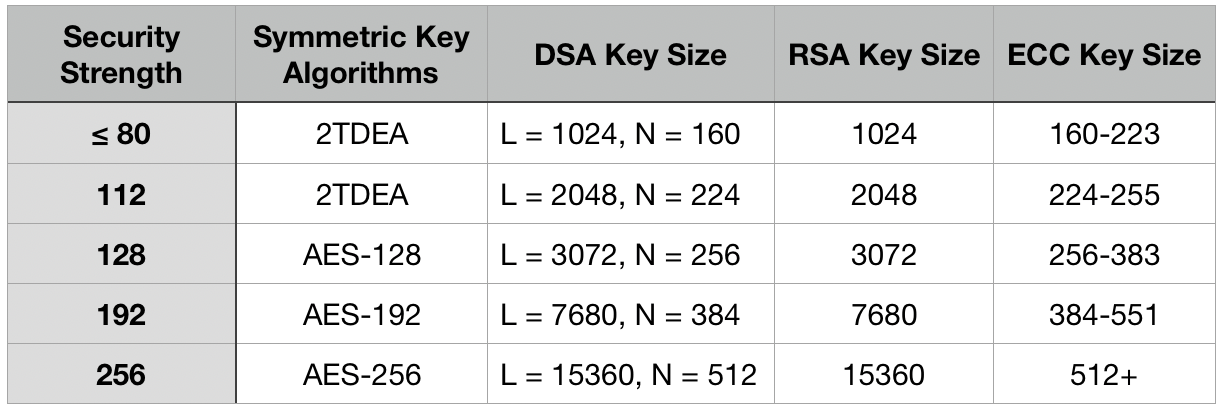
\includegraphics[scale=0.4]{NIST_Comparable_Strengths.png}
\caption{\small{NIST Comparable Key Strengths}}
\label{fig:NIST_Comparable_Strengths}
\end{figure}

\begin{figure}
\centering
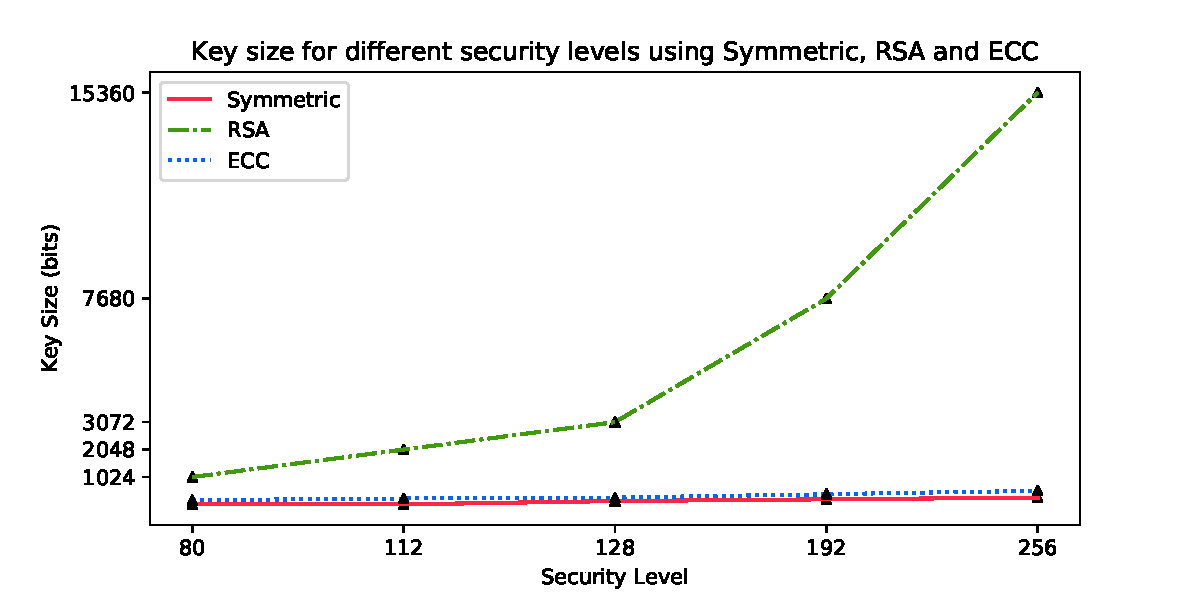
\includegraphics[scale=0.45]{NIST_KeySize_Compare_Security_Strength}
\caption{\small{NIST key size requirement for different security strength using Symmetric, RSA and ECC}}
\label{fig:NIST_KeySize_Compare_Security_Strength}
\end{figure}

\noindent \textbf{Speed Performance}

Our objective is to observe how ECDSA performs with different key sizes in Key Generation, Message Signing and Signature Verification process. Several choices have to be made before implementing an ECDSA system, including selection of elliptic curve domain parameters, algorithms for elliptic curve arithmetic, protocol arithmetic and field arithmetic. 

In our experiment, we use FIPS 186-4 \cite{Kerry13fipspub} revised by NIST to include ECDSA as specified in ANSI X9.62. We use five prime fields and one randomly selected elliptic curve for each fields recommended by NIST FIPS 186-4. The curves are denoted as $p192$, $p224$, $p256$, $p384$, $p521$. 
\begin{align*}
    & p192 = 219^{2} - 2^{64} - 1 \\
    & p224 = 2^{224} - 2^{96} - 1 \\
    & p256 = 2^{256} - 2^{224} + 2^{192} + 2^{96} - 1 \\
    & p384 = 2^{384} - 2^{128} + 2^{96} + 2^{32} - 1 \\
    & p521 = 2^{521} - 1
\end{align*}

Since those curves use different key sizes, we can do the experiment with them to observe the speed performance of varying key sizes. Additionally, for the 256 bit size we add another curve $secp256k1$ defined in Standards for Cryptography (SEC), since it is used in Bitcoin public-key cryptography. Unlike other NIST Curves, $secp256k1$ was constructed in a predictable and non-random way, which makes the computation more efficient. The dataset we used is the file that contains 6000 lines of messages. And the implementation we used is FastECDSA, which will be discussed further in Implementation session. Figure~\ref{fig:ECDSA_Varying_Keysize_Runtime_Graph} and Figure~\ref{fig:ECDSA_Varying_Keysize_Runtime_Table} table show the experiment result of ECDSA Performance under Different Elliptic Curves (Key sizes).

\begin{figure}
\centering
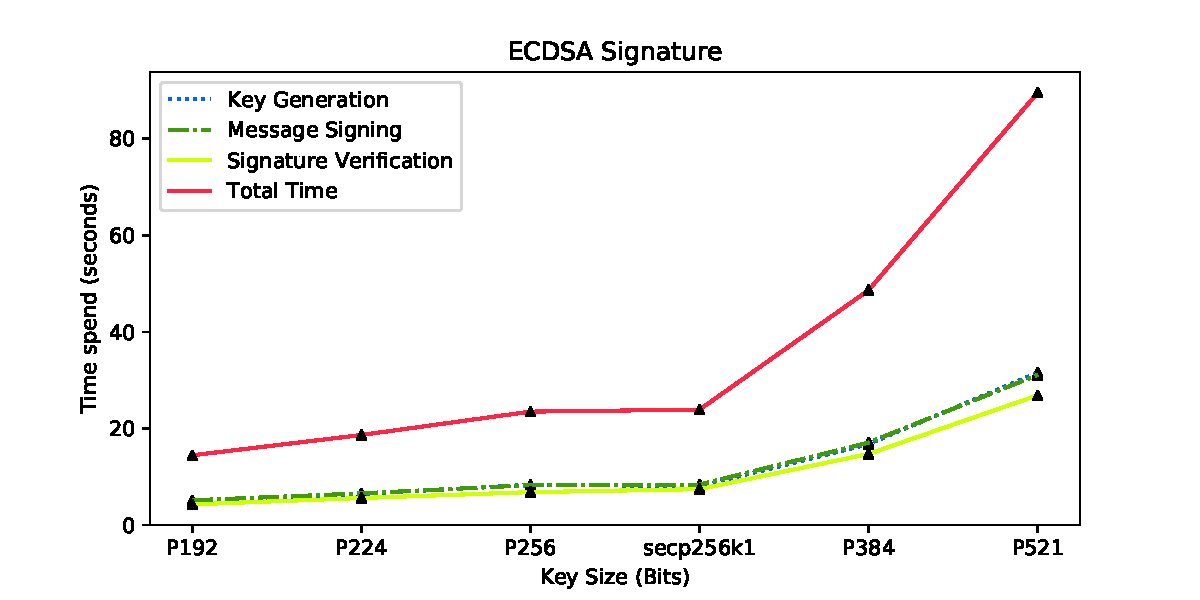
\includegraphics[scale=0.45]{ECDSA_Varying_Keysize_Runtime_Graph}
\caption{\small{ECDSA performance under different Elliptic Curves with fixed message size 6000}}
\label{fig:ECDSA_Varying_Keysize_Runtime_Graph}
\end{figure}

From the table and graph, we observed that for each individual curve, the time for performing all three stages in ECDSA are fairly the same. For smaller key sizes from 192 to 256, the time for generating, signing and verifying differ only a little. After size 256, time for the three stages grows significantly. 
\\
\\
\noindent \textbf{RSA vs ECDSA}

Tables in Figure~\ref{fig:new_evr_gen}, \ref{fig:new_evr_sign}, \ref{fig:new_evr_veri} compare the time using for Key Generation, Message Signing, Signature Verification with comparable key sizes for ECDSA and RSA. We use message size of 1 (i.e. signing and verifying 1 line of message). Both implementations of the two digital signature schemes are using OpenSSL and the same one message to ensure the comparability. We draw those data in Figure~\ref{fig:EVR_overall} to see the trends. From the result, ECDSA outperforms RSA in Key Generation and Message Signing stages, but underperforms RSA in Signature Verification stage. To reach the same security level in Key Generation stage, the 15360 bits RSA has to take 66.67 seconds while 512 bits ECDSA only takes 0.14 seconds, significantly faster. In Message Signing stage, at the beginning RSA is faster than ECDSA. As the key sizes increasing, however, ECDSA speeds up and surpasses RSA and RSA slows down. Finally, when the key size is very large, ECDSA still outperforms RSA a lot. In the Signature Verification stage, ECDSA takes considerably much longer time than RSA. And for the small key size, the time used by RSA for the verification are barely changed as the key sizes increasing.

\begin{figure*}
\centering
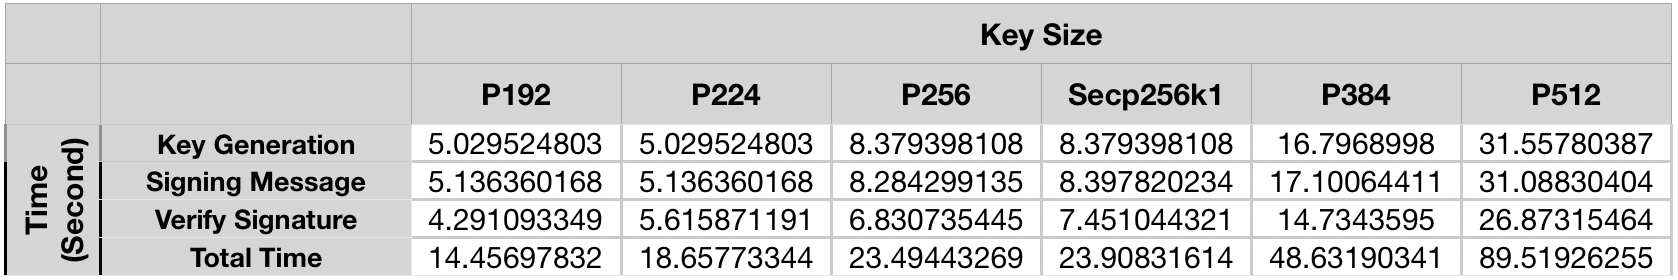
\includegraphics[scale=0.45]{ECDSA_Varying_Keysize_Runtime_Table}
\caption{\small{ECDSA performance under different Elliptic Curves with fixed message size 6000}}
\label{fig:ECDSA_Varying_Keysize_Runtime_Table}
\end{figure*}

\begin{figure}[H]
\centering
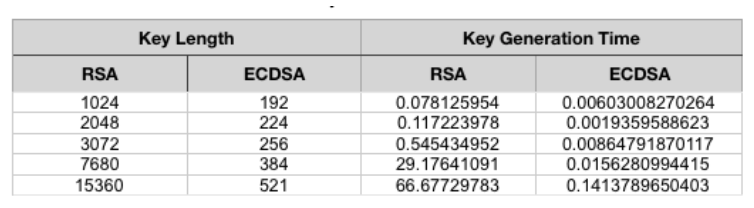
\includegraphics[scale=0.62]{new_evr_gen}
\caption{\small{Key Generation Time for RSA vs ECDSA}}
\label{fig:new_evr_gen}
\end{figure}

\begin{figure}[H]
\centering
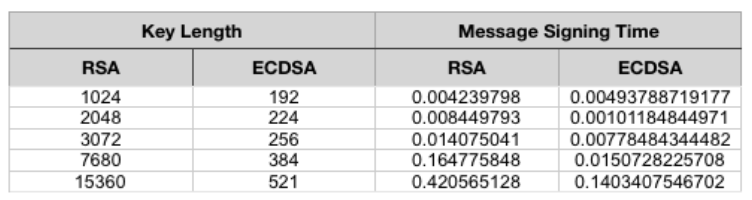
\includegraphics[scale=0.62]{new_evr_sign}
\caption{\small{Message Signing Time for RSA vs ECDSA}}
\label{fig:new_evr_sign}
\end{figure}

\begin{figure}[H]
\centering
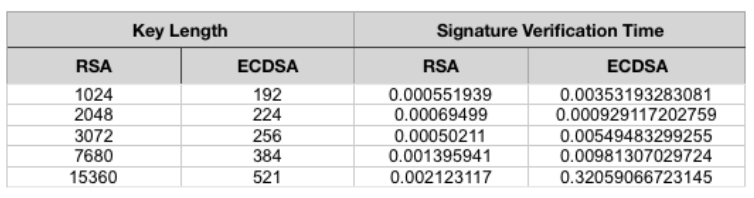
\includegraphics[scale=0.62]{new_evr_veri}
\caption{\small{Signature Verification for RSA vs ECDSA}}
\label{fig:new_evr_veri}
\end{figure}


% \begin{figure}[H]
% \centering
% 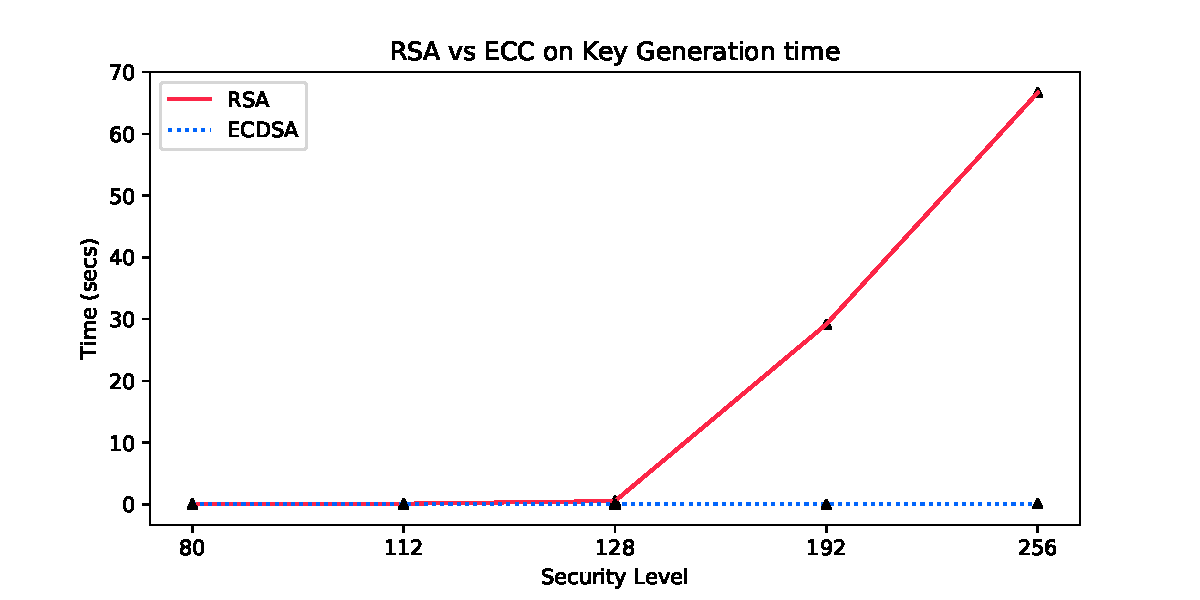
\includegraphics[scale=0.45]{ECDSA_RSA_Compare_KeyGen_Graph}
% \caption{\small{Key Generation Time for RSA vs ECDSA}}
% \label{fig:ECDSA_RSA_Compare_KeyGen_Graph}
% \end{figure}

% \begin{figure}[H]
% \centering
% 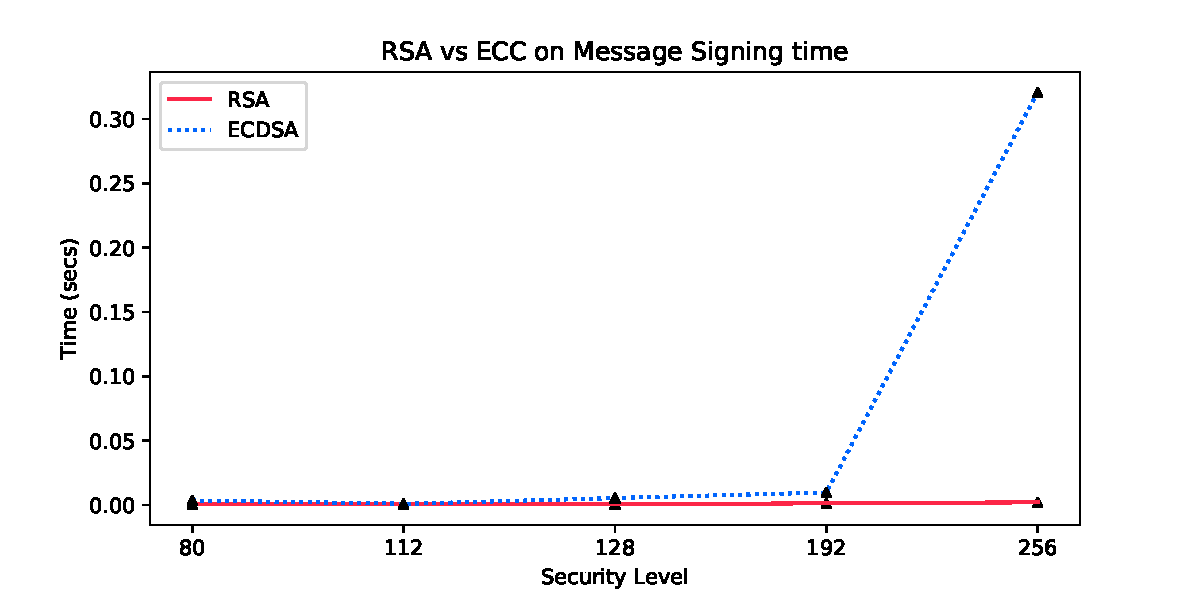
\includegraphics[scale=0.45]{ECDSA_RSA_Compare_Signing_Graph}
% \caption{\small{Message Signing Time for RSA vs ECDSA}}
% \label{fig:ECDSA_RSA_Compare_Signing_Graph}
% \end{figure}

% \begin{figure}[H]
% \centering
% 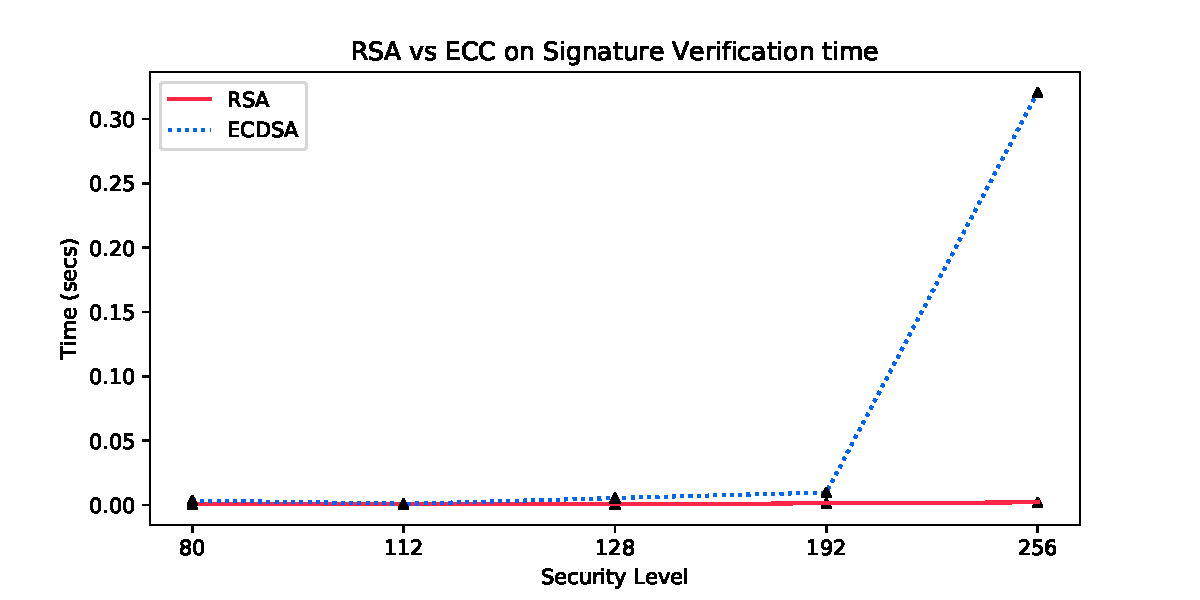
\includegraphics[scale=0.45]{ECDSA_RSA_Compare_Verification_Graph}
% \caption{\small{Signature Verification for RSA vs ECDSA}}
% \label{fig:ECDSA_RSA_Compare_Verification_Graph}
% \end{figure}

\begin{figure*}
\centering
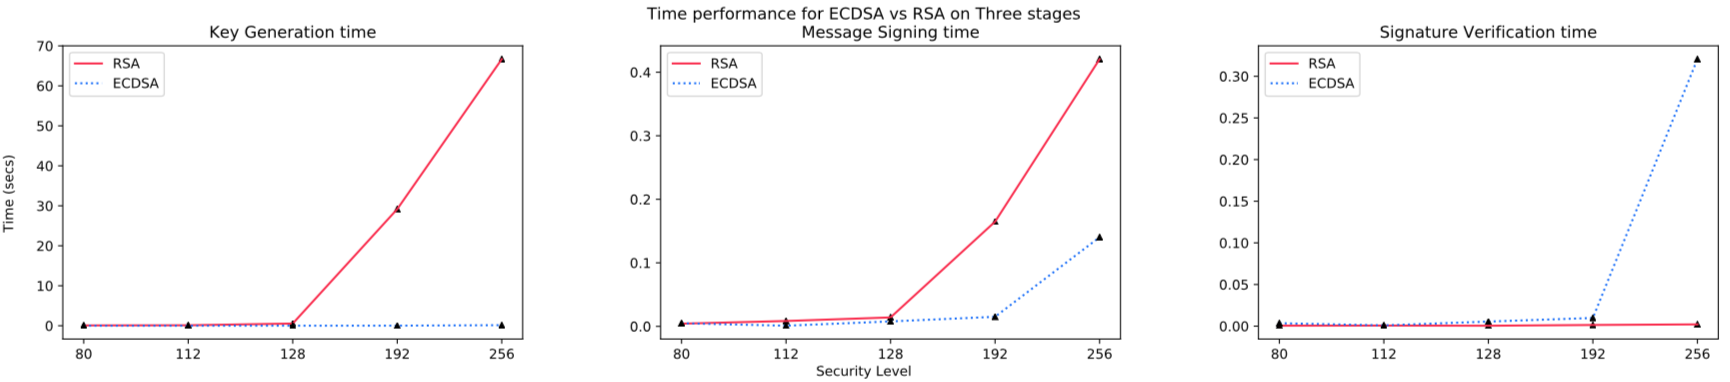
\includegraphics[scale=0.5]{EVR_overall}
\caption{\small{Time Performance for ECDSA vs RSA on Three Stages }}
\label{fig:EVR_overall}
\end{figure*}

From the above analysis we can conclude that ECDSA with the smaller key size can save a lot of resources such as time and space storage, which is better than RSA. RSA can be used in the case when the receiver needs to verify more messages than the number that are produced. 
\\
\\
\noindent \textbf{Implementation Method}

We use three different packages found online to implement ECDSA process. The first one is implemented purely in Python and released under the MIT license \cite{BrianWarnerECDSA}. When trying to use this package to implement ECDSA, we find out it takes significantly longer time to all of the three stages. Then, we explore online and decide to adopt the second approach, FastECDSA, which is implemented in C \cite{AntonKueltzECDSA}. For third method, we use the python cryptography library that has OpenSSL backend \cite{PyCACryptography}. As shown in Figure~\ref{fig:ECDSA_Implementation_Compare_Steps}, the pure python package takes substantially much time than the other two approaches, especially in Key Generation and Signature Verification stages. The package that uses OpenSSL has the best performance in all stages.

\begin{figure}[H]
\centering
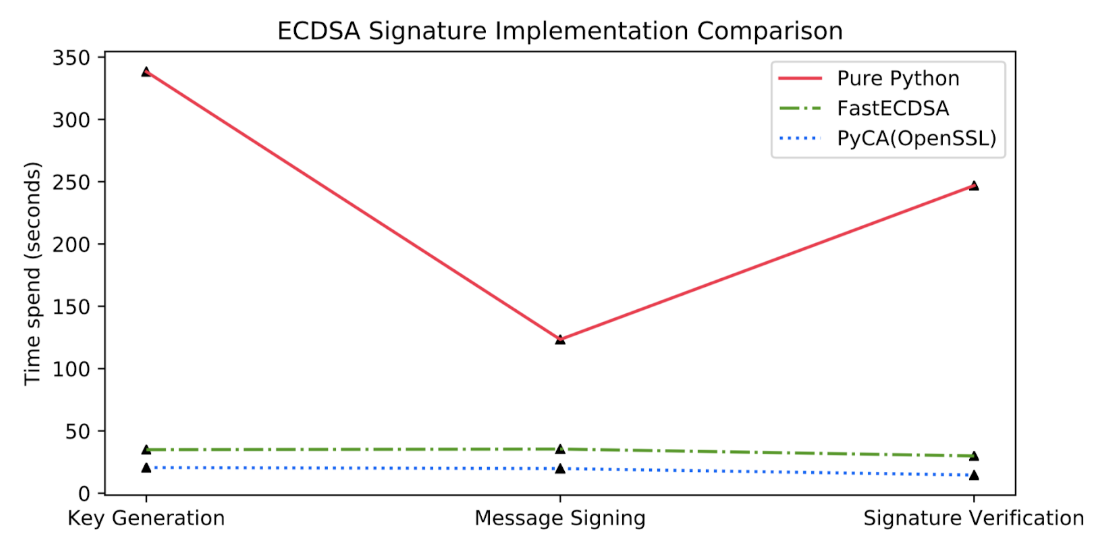
\includegraphics[scale=0.45]{ECDSA_Implementation_Compare_Steps}
\caption{\small{ECDSA Performance under Different Implementation}}
\label{fig:ECDSA_Implementation_Compare_Steps}
\end{figure}

\subsection{Security Considerations}

The most important security considerations when using ECDSA is to against the chosen-message attack. Attacker obtains the sender's signature on a collection of messages (excluding $m$) and his goal is to obtain a valid signature on a single message $m$. We classify the possible attacks into three categories as follows. 
\\
\\
\noindent \textbf{Per-message Secrets}

One attack in Signature Generation stage is related to the per-message secrets $k$. If the same secret $k$ is using many times, attackers can easily break ECDSA and obtain the entities' secret keys. The mechanism is shown in Breaking ECDSA Algorithm~\ref{algo:Breaking_ECDSA} below.

\begin{algorithm}
\begin{algorithmic}
\STATE Breaking ECDSA with static per-message secret $k$
\STATE $s1 \gets k^{-1}(z1 + r \times dA) \mod n$
\STATE $s2 \gets k^{-1}(z2 + r \times dA) \mod n$
\STATE $s1 - s2 = k^{-1}(z1 - z2) \mod n$
\STATE $k = (s1 - s2)^{-1} (z1 - z2) \mod n$ 
\end{algorithmic}
\caption{Breaking ECDSA}
\label{algo:Breaking_ECDSA}
\end{algorithm}

Sony Corporation used a static $k$ as the secret to generate all the signatures in August 2013. Initially only the signed games can run on PS3 game console. After the attacker break ECDSA and recover the secret key, everyone can play every games. This issue can be avoided by destroying after each message is signed.
\\
\\
\noindent \textbf{ECDLP Attacks}

To ensure ECDSA is secure, the elliptic cryptography discrete logarithm problem (ECDLP) cannot be easily solved. It is defined in Key Generation stage as solving for $d$ in $Q=dG$. Within many known attacks against ECDLP, there are four very famous ones. Exhaustive search, Pohlig-Hellman, Pollard-rho and Multiple logarithms, which are described details in \cite{johnson2001elliptic}. 
\\
\\
\noindent \textbf{Other Attacks}

The hash function that is used to encrypt the original message is better to be collision resistant. Traditional hash function such as SHA-1 is not collision resistant nor preimage resistant, thus are weak to the attackers. Implementation attacks such as timing attacks and differential fault analysis could happen as well.



%%% ECDSA END


%%% EdDSA START

\section{EdDSA}

Edwards-curve Digital Signature Algorithm (EdDSA) is a digital signature scheme based on (possibly twisted) Edwards curves, which is a variant of Schnorr's signature system. It has been proven to provide high performance over a variety of platforms and be securer because it is more resilient to side-channel attacks (including timing attack etc.) and provides collision resistance as well (only holds for PureEdDSA). Also, it is space efficient since it only requires small public/private key pair (32 or 57 bytes) and produces short signatures (64 or 114 bytes) and can achieve around 128-bit and 224-bit security level separately.

\subsection{Parameters}

General EdDSA signature scheme has 11 parameters.

\begin{enumerate}
    \item $p$, an odd prime and EdDSA exploits an elliptic curve on the finite field $GF(p)$.
    \item $b$, EdDSA uses $b$ bits for public/private keys and produces $2*b$ bits for signature and $2^{(b-1)} > p$.
    \item $(b-1)$-bit encoding of elements of $GF(p)$.
    \item $H$, a hash function that produces $2*b$-bit output.
    \item $c$, co-factor of base-2 logarithm.
    \item $n$, secure EdDSA schemes have $n+1$ bits with $c \leq n < b$.
    \item $d$, non-square element of $GF(p)$, which is always nearest to zero.
    \item $a$, non-square element of $GF(p)$, which would be 1 if $p \mod 4 = 1$ and; -1 if $p \mod 4 = 3$.
    \item $B$, an element from $set\{(x,y)\}$, a member of $GF(p)*GF(p)$ where $a * x^2 + y^2 = 1 + d * x^2 * y^2$.
    \item $L$, an odd prime which $[L]B = 0$ and $2^c * L = \#E$, where $\#E$ is the number of points on the curve).
    \item $PH$, pre-hash function which generates a fixed length of message before getting into EdDSA scheme, where $PH(M) = M$ means no pre-hash function.
\end{enumerate}

Ed25519 has been chosen for our experiment since it is most widely used instance of EdDSA and supposed to provide a 128-bit security level, which is perfectly safe and can defeat many side channel attacks as a PureEdDSA. It takes SHA-512 as hash function and no pre-hash function, and exploits Curve25519 where:
\begin{align*}
-x^2 + y^2 = 1 - 121665/121666(x^2y^2)    
\end{align*}

\subsection{Algorithm}
EdDSA uses a $b$-bit long private key and a hash function $H$, producing a $2b$-bits output. One of the most common hash function used here is SHA-512 (b = 256), which is used by Ed25519. $H(k)$ can be represented as $(h_0,h_1,\dots,h_{2b-1})$. Therefore, the signing process of message $M$ can be expressed as shown in Algorithm~\ref{algo:EdDSA_Algorithm} where $A$ is the public key and $B$ is the base point of order $l$ and $A=a \cdot B$

\begin{algorithm}
\begin{algorithmic}
\STATE \textbf{Input}: $M$,$(h_0,h_1,\dots,h_{2b-1})$, $B$ and $A$ \\
\quad 1. $a \gets 2^{b-2} + \sum_{3\leq i \leq b-3} 2^i h_i$ \\
\quad 2. $h \gets H(h_b,\dots,h_{2b-1},M)$ \\
\quad 3. $r \gets h \mod l$ \\
\quad 4. $R \gets r \cdot B $ \\
\quad 5. $h \gets H(R,A,M)$ \\
\quad 6. $S \gets (r+ah) \mod l$
\\
\textbf{return} $(R,S)$
\end{algorithmic}
\caption{EdDSA Algorithm}
\label{algo:EdDSA_Algorithm}
\end{algorithm}


\noindent For verifying, a signature should be valid if $R \in E, S \in \{0,1,\dots,l-1\}$ and meet the equation:
\begin{align*}
    8S \cdot B = 8 \cdot R + 8H(R,A,M) \cdot A
\end{align*}

\noindent And it can be shown that it takes much harder mathematics computation to verify a signature.


\subsection{Performance}

\begin{figure}[H]
\centering
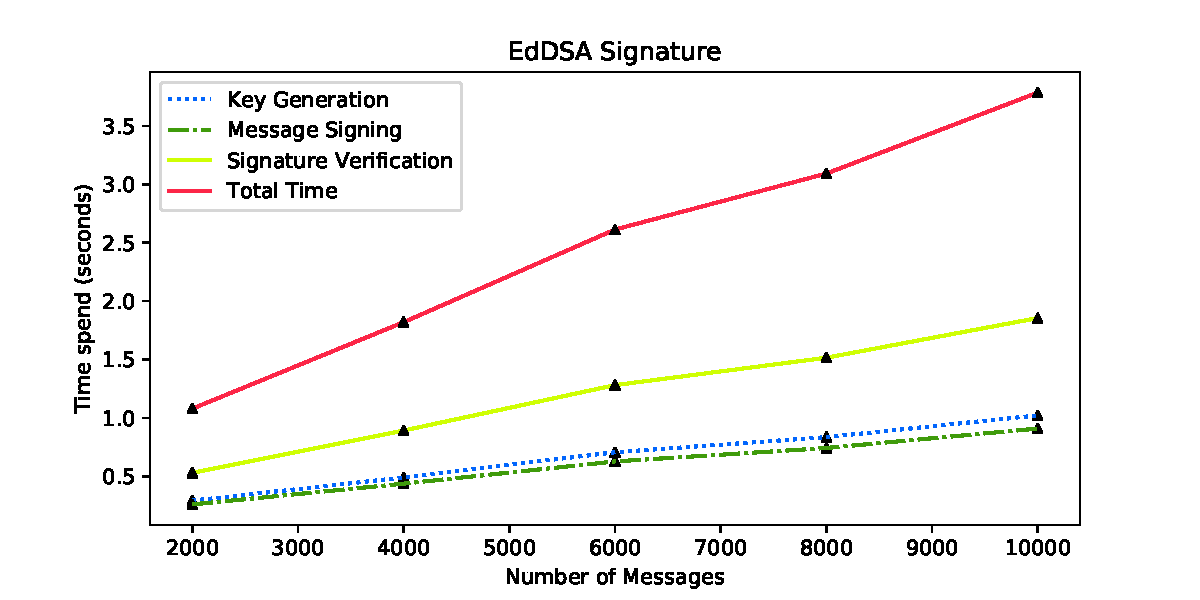
\includegraphics[scale=0.45]{EdDSA_Performance_Runtime}
\caption{\small{EdDSA Performance Runtime}}
\label{fig:EdDSA_Performance_Runtime}
\end{figure}

Unlike RSA and ECDSA which can alter parameters to evaluate the performance, the EdDSA algorithm has fixed parameters once we decided to apply Ed25519 in the experiments. Therefore, our focus of EdDSA's performance is on the time it takes in different stages (key generation, sign, verify). As depict in Figure~\ref{fig:EdDSA_Performance_Runtime}, it takes only at most ~4 seconds for 10000 messages. The runtime benchmarking shows in Figure~\ref{fig:EdDSA_Performance_Runtime} uses the PyNaCL \cite{PyNaCl} implementation that run over varying messages of 2000, 4000, 8000 and 10000 (i.e. varying load).  Since it is very fast algorithm, we run with varying messages to observe sensible performance measure.

Furthermore, we found three implementations for EdDSA and intended to figure out how different implementation might affect the performance. The first one we found is ed25519 python package, provided by Brain Warner \cite{BrianWarner}, it is a simple and straightforward implementation, however, it consumes much time on our testing environment. Then, we found two other python packages PyNaCL \cite{PyNaCl} and LibNaCL \cite{libnacl}, which also provide ed25519 signature algorithm, but much faster implementation. We compared these three implementations with varying message length and record total time of key generation, signing all messages and verifying all signatures and experiment details are shown in Figure~\ref{fig:EdDSA_Implementation_Compare_Total} and table in Figure~\ref{fig:EdDSA_Implementation_Compare_Total_Table}.

\begin{figure}
\centering
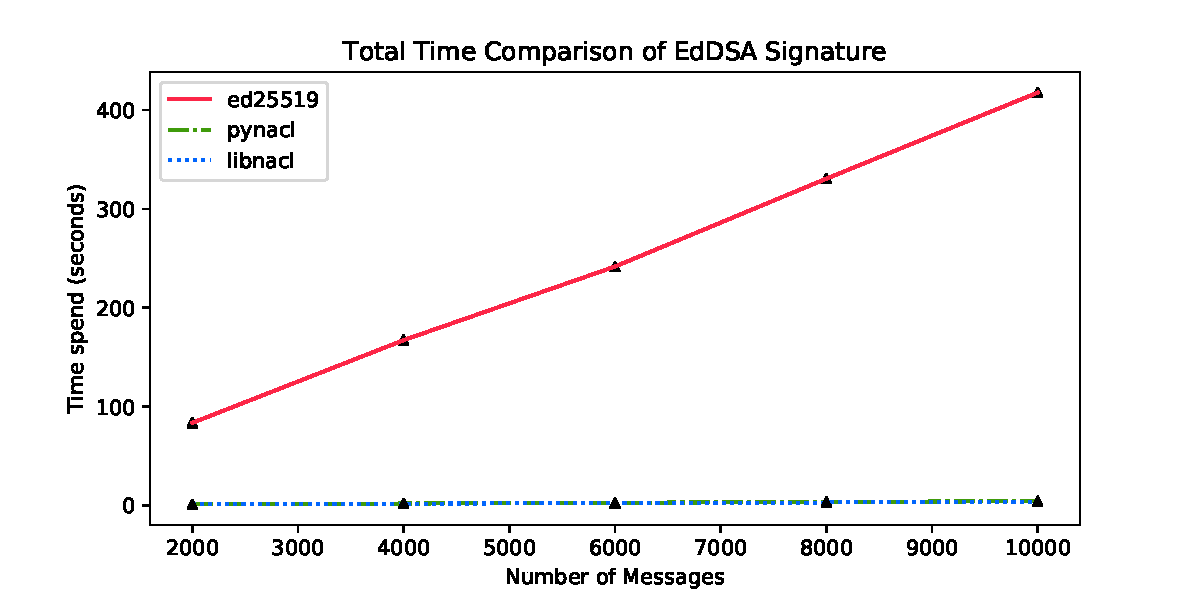
\includegraphics[scale=0.45]{EdDSA_Implementation_Compare_Total}
\caption{\small{Total Time of EdDSA Implementations}}
\label{fig:EdDSA_Implementation_Compare_Total}
\end{figure}

\begin{figure}
\centering
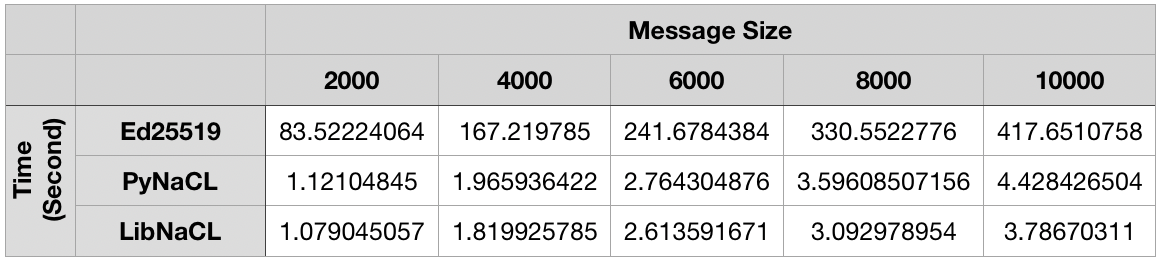
\includegraphics[scale=0.4]{EdDSA_Implementation_Compare_Total_Table}
\caption{\small{Total Time of EdDSA Implementations Table}}
\label{fig:EdDSA_Implementation_Compare_Total_Table}
\end{figure}

It is clear that all three implementations' total execution time grows almost linearly with input size increasing, which means input size has no influence with the individual execution time for each message no matter what implementation is applied.

Besides, ed25519 package takes much more time than the other two packages, therefore, different implementations do have big influence in terms of total time even though we can be sure that we all implement same algorithm (provide same level security), because they all just offer a python interface to a C implementation of Ed25519 public key signature system (\url {http://ed25519.cr.yp.to}) and refer to original paper \cite{Bernstein2012}, provided by creators of this algorithm, Bernstein et al. 

So as to understand how much each step contributes to the total time for three implementations, we used the fixed message size of 6000 lines (i.e. fixed load), and evaluated execution times for each implementation as shown in Figure~\ref{fig:EdDSA_Implementation_Compare_Steps}. It is obvious that key generation and signing processes almost take the same amount of time, however, verifying process takes much more time than these two, which is two to three times longer. As we analysed before, the verifying process needs much more complicated mathematics computation, thus, it is reasonable that it takes much longer time.

\begin{figure}
\centering
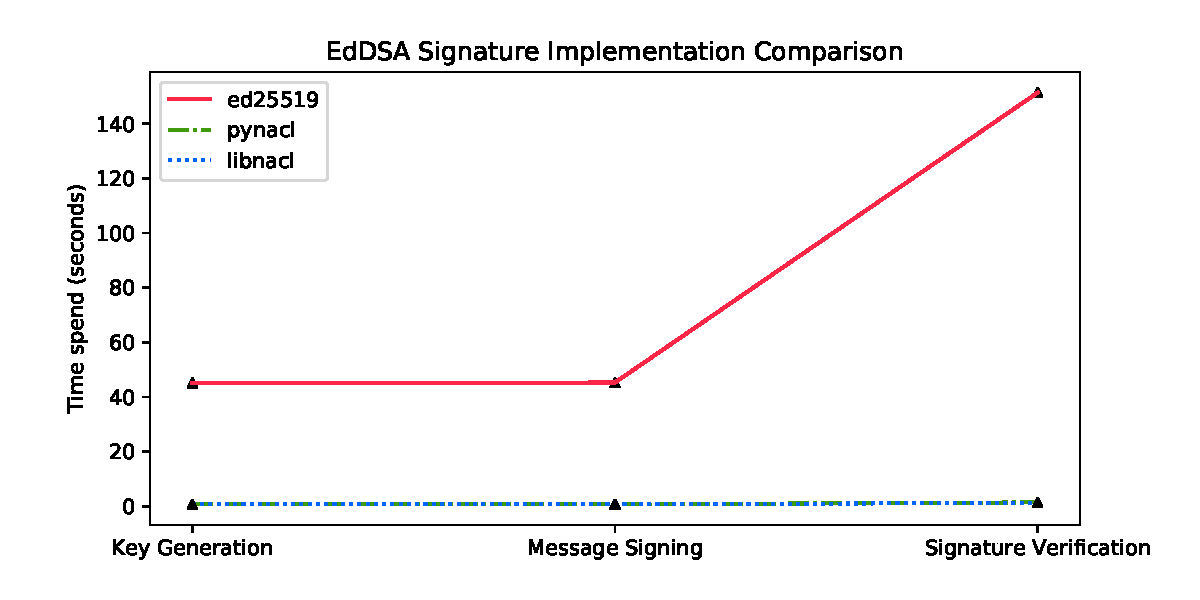
\includegraphics[scale=0.45]{EdDSA_Implementation_Compare_Steps}
\caption{\small{Steps comparison of EdDSA implementations over fixed message size 6000}}
\label{fig:EdDSA_Implementation_Compare_Steps}
\end{figure}

\subsection{Security}

EdDSA is proven to provide better security thanks to nice properties of twisted Edwards curves it works over. Particularly, Ed25519 exploits the Montgomery curve ``Curve25519", which does not apply branch operations or array indexing steps which depend on secret data to implement its scalar multiplication, in order to avoid many side channel attacks \cite{8167706}.

However, it might still be vulnerable to fault attacks. In \cite{8167706}, they perform a valid attack on the signing algorithm above and proposed a fault algorithm as shown in Algorithm~\ref{algo:EdDSA_Fault_Algo}.

\begin{algorithm}
\begin{algorithmic}
\STATE Input: M, A, (R, S) and (R, S')
\STATE $h \gets H(R, A, M)$ 
\STATE $i \gets 0$
\FOR {i < 32}
    \STATE $e \gets  1$
    \FOR {e < 256} 
        \STATE $h' \gets  2^{8i} e \oplus h$
        \STATE $a \gets (S - S')(h - h')^{-1} \mod l$
        \IF{$a \cdot B == A$}
        \RETURN a
        \ENDIF
        \STATE $e \gets  e + 1$
    \ENDFOR
    \STATE $i \gets i + 1$
\ENDFOR
\RETURN ERROR
\end{algorithmic}
\caption{Fault Algorithm to attack on EdDSA}
\label{algo:EdDSA_Fault_Algo}
\end{algorithm}

Then, they found that by selecting $r$ as a random number, they can compute a new $(R, S)$ as a signature for the message M where the equation would be:

\begin{align*}
    8S \cdot B = 8(r + H(R,A,M) a) \cdot B = 8 \cdot R + 8H(R,A,M) a \cdot B \\
    = 8 \cdot R + 8H(R,A,M) \cdot A
\end{align*}


Therefore, the verifying equation still holds for this, which means we can forge valid signatures for messages. It illustrates that EdDSA is still vulnerable to fault attacks, and protections or countermeasures against them should be considered if the algorithm is applied in areas where fault attacks are possible.

%%% EdDSA END


%%% Lamport START

\section{Lamport Signature Scheme}

Lamport one-time signature scheme is an efficient method for constructing digital signature, which can resist quantum computing. The currently used digital signature schemes rely on the algorithmic complexity which is fragile when confronting quantum computer. Lamport signatures can be built from any cryptographically secure one-way hash function. Strength of Lamport signature, however, depends on the strength of hash function it utilized in implementation.

\subsection{Implementation Details}

The Lamport signature scheme performs its working in three steps. 

\vspace{0.5em}

\noindent\textbf{Keys Generation:} \quad Use random number generator to produce 256 key pairs of random numbers as private key, each number is 256 bits, total 16 KiB. The public key is the corresponding hash value (SHA256) of private key, thus implementing 512 hashes, each 256 bits in size, public key has same size with private key.\\

\noindent\textbf{Message Signing:} \quad Create a 256-bit hashsum of the message. For each n-th bit in the hashsum, pick a corresponding number from the private key. For example, if the n-th bit is 0, pick an n-th number in the first row, if the n+1th bit is 1, pick the n+1th number from the second row. This way produces 256 numbers each of 256 bits, the signature size is total 8 KiB.\\

\noindent\textbf{Signature Verification:} \quad Create a 256-bit hashsum of the message. Pick the corresponding public key for each bit, then calculate hash value of each number in signature. If hash values are same as the values picked from public key, it indicates the message received is original, otherwise, the message or signature has been tampered during the transmission or does not belong to sender. 
\vspace{0.5em}

\noindent The Figure~\ref{fig:Lamport_Implementation_Details} illustrates every step.

\begin{figure}[H]
\centering
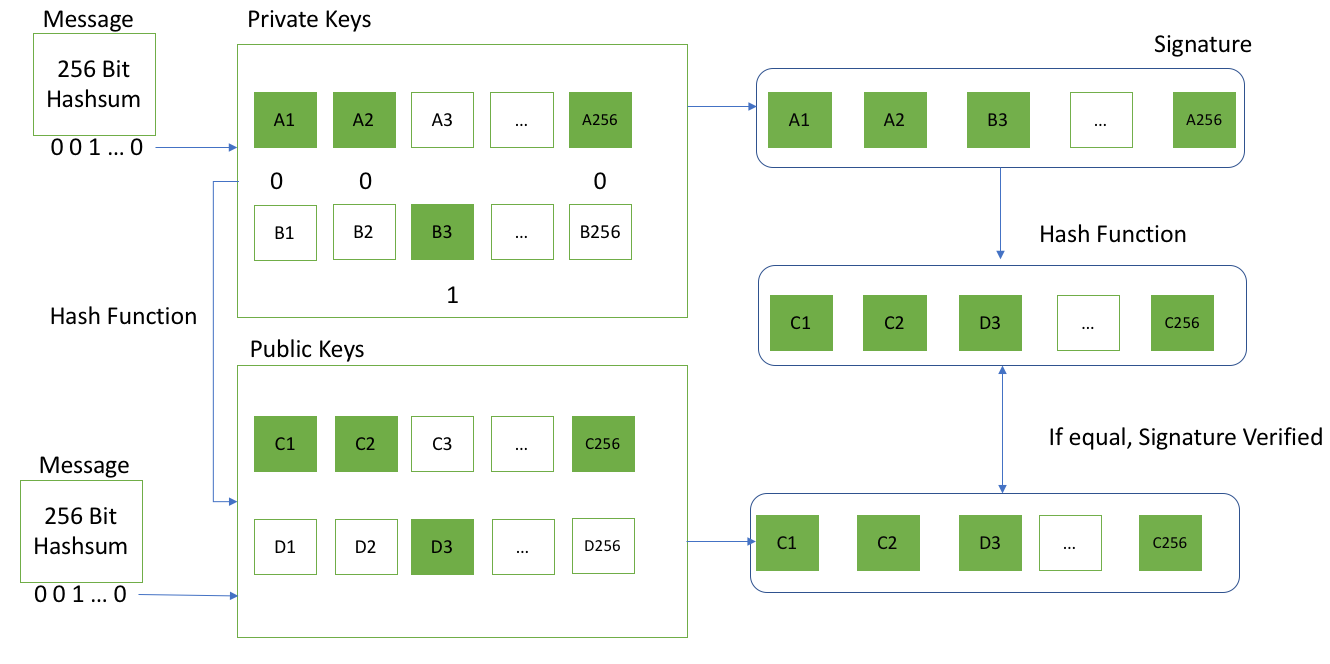
\includegraphics[scale=0.18]{Lamport_Implementation_Details.png}
\caption{\small{Implementation of Lamport Signature Scheme}}
\label{fig:Lamport_Implementation_Details}
\end{figure}


\subsection{Mathematical Notation}

\textbf{Keys:} \quad Let $k$ be a positive integer and let $m = \{0,1\}^k$ be the hashsum of the message. Let $f:Priv \to Pub$ be a one way hash function. For $1 \leq i \leq k$ and $j \in \{0,1\}$, the sender computes hash value of each random number $Priv_{i,j}$, and get $Pub_{i,j} = f (Priv_{i,j})$. The size of private key is 2k, the size of public key is 2k as well.
\\
\\
\noindent \textbf{Signing a message:} \quad Let $m = m_1 \dots m_k \in \{0,1\}^k$. The signature of the message is:
\begin{align*}
sig(m_1 \dots m_k) = (Priv_{1,m1,}, \dots , Priv_{k,mk}) = (s_1, \dots, s_k)    
\end{align*}

\noindent \textbf{Verifying a signature:} \quad Receiver validates a signature by checking $f(s_i)= Pub_{i,mi}$, for all $1 \leq i \leq k$.

\subsection{Characteristics}

\textbf{Strength:} \quad An important factor in the strength of Lamport signature scheme is flexible. If a hash function that is employed with the scheme is proven to be weak, it can easily be replaced with another strong hash function. The common hash used in Lamport signature scheme is SHA256, which is proved as secure in most scenarios.

Lamport signature scheme is quantum resistant due to a large number of hash functions it employees in its implementation. Other digital signature schemes such as RSA, ECC, whose credibility depends on their algorithm complexity. They are much prone to be broken by quantum computer \cite{8346359}. The increasing development towards a practical computer is a threat to such signature schemes.

Lamport signature scheme costs less time than traditional signature scheme based on public key cryptography. It is suitable to apply on the resource-constrained devices like IoT devices.
\\
\\
\noindent \textbf{Weakness:} \quad Large computation and storage requirements are the main limitations of Lamport signature. For example, sender randomly generates 256 pairs of 256-bit numbers as private key, the total size of these pairs equals $2*256*256=16$ KiB. Sender needs to calculate 512 times hash of private key then get corresponding public key, which has same size 16KiB. The signature's size is the half of private key or public key, that is 8KiB. Compared to other signature scheme like RSA, the signature size is relatively large. Similarly, receiver needs to calculate 256 times hash of signature in verification process. Besides, this is one time scheme, key pairs cannot be used next time. It indeed requires a large memory to store these key pairs in signing process. Lamport signature scheme puts more loads on devices' storage and computation compared with traditional signature schemes \cite{8402796}.

The key pair can be only used to sign one message each time. If there are multiple messages to be signed, many key pairs have to be generated for a safety purpose. 

\subsection{Experiment}

The objective of this experiment is to measure the execution time of Lamport Signature algorithm and find which step costs most of time. The program was written in Python, and no package was used. The test data set includes three different size csv files, which are 1000 entries, 5000 entries and 10000 entries. The default hash function is SHA256. The execution time of the program is as shown in Figure~\ref{fig:Lamport_Runtime_Table} table.

\begin{figure}[H]
\centering
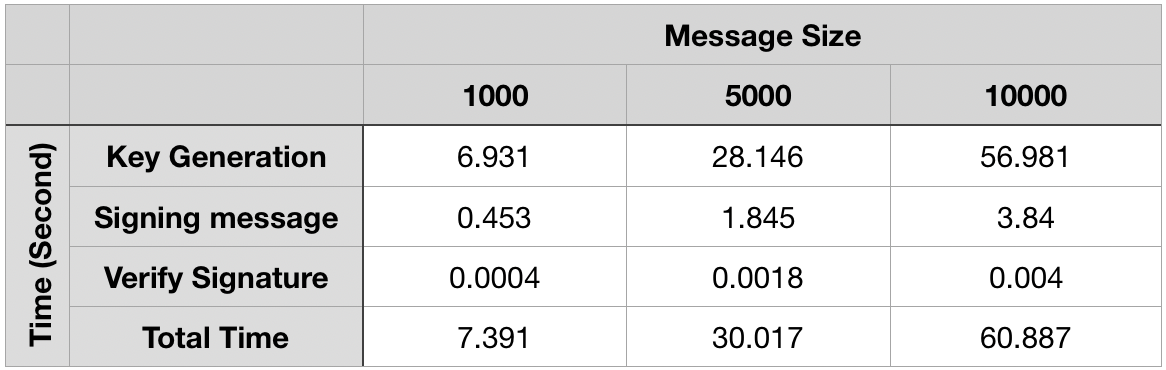
\includegraphics[scale=0.4]{Lamport_Runtime_Table.png}
\caption{\small{Lamport Runtime Table}}
\label{fig:Lamport_Runtime_Table}
\end{figure}

\begin{figure}[H]
\centering
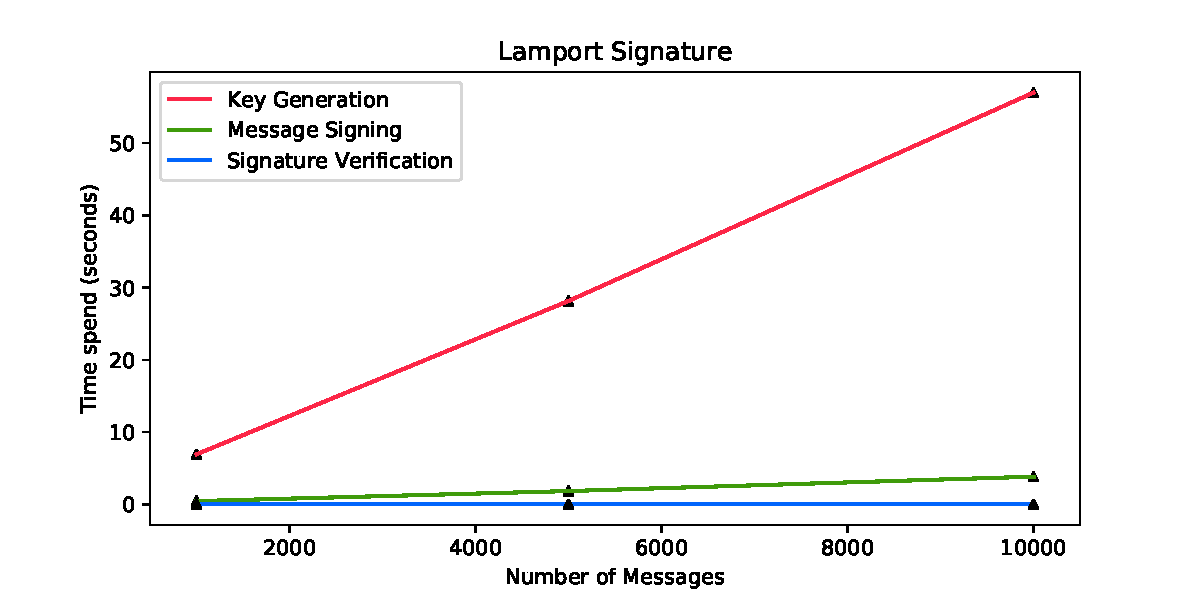
\includegraphics[scale=0.45]{Lamport_Runtime_Graph}
\caption{\small{Lamport Runtime Graph}}
\label{fig:Lamport_Runtime_Graph}
\end{figure}

From the chart in Figure~\ref{fig:Lamport_Runtime_Graph}, we can observe that  key generation accounts for large part of time, nearly 90\% of total time, the performance of Lamport signature scheme is dominated by key generation time. Because large amount of hash calculations are in key generation step, for this case, there are 512 random numbers in public key, so there are total 512 times SHA256 calculations. While in sign message step, the program only calculates the hashsum of message. In verifying step, the program only calculates 256 times SHA256. Therefore, it is obvious that key generation is the most time-consuming step in Lamport signature.

\subsection{Security Analysis}

The security performance of Lamport signature is dominated by its hash function. For a hash function that generates an n-bit message digest, according to Grover's algorithm \cite{8463331}, finding a pre-image collision on a single invocation of an ideal hash function is upper bound on $Ο(2^{n/2})$ operations under a quantum computing model. For each private key and its corresponding public key pair in Lamport signature, the private key length must be selected so performing a pre-image attack on the length of the input is not faster than performing a pre-image attack on the length of the output. For example, if each private key element was only 16 bits in length, it is trivial to exhaustively search all $2^{16}$ possible private combinations in $2^{16}$ operations to find a match with the output. Based on Grover's algorithm, a quantum secure system, the length of the public key elements and private key elements and the signature elements must be no less than 2 times larger than the security rating of the system \cite{4897262}. An 80-bit secure system uses element lengths of no less than 160 bits, a 128-bit secure system uses element lengths of no less than 256 bits. SHA256 is commonly used in Lamport signature, SHA512 is much safer but at the cost of longer key generating time and larger signature size. 

\subsection{Improvement}

Large computation and storage requirement in Lamport's key generation process are the main disadvantages of this scheme. Other one-time signature schemes like Merkle, HORS, Merkle-Winternitz improve Lamport efficiently, even if they all have their pros and cons. For example, each Lamport public key can only be used to sign one single message, which means many keys have to be published if many messages are to be signed, Merkle tree structure can be used for these public keys, only publishing the top of the hash tree instead, a single hash can be used to verify any given number of future signatures, this mechanism indeed decrease key storage requirement.


%%% Lamport END


%%% Cross Comparsion START

\section{Cross Comparison Analysis}

To evaluate performance between RSA, ECDSA, EdDSA and Lamport digital signature schemes, we perform the cross comparison runtime analysis of these algorithms with their fixed "ideal" setting. Here, the "ideal" setting, we mean that the best performance to security ratio and trade-off. However, we also note that it is still challenging to justify the ideal setting because some of these algorithms work quite differently in their mathematical foundation, pre-processing and algorithmic steps. Table in Figure~\ref{fig:Cross_Compare_Label} summarise the setting and parameter of each algorithm and, we label them $A1 \dots A8$ accordingly. We highlight that even though we do not review particularly to the Digital Signature Algorithm (DSA), but we include DSA in our runtime performance analysis to observe better for the purpose of supplementing stronger argument for ECDSA runtime. The justification of the "ideal" setting is based on our best effort evaluating each algorithm by a combination of our collaborative investigation and, by reviewing a couple of related literature as cited in references.

\vspace{0.5em}

\noindent Our quantitative performance measurement methodology works as follows:

\begin{enumerate}
    \item We prepare test dataset in 10 CSV files: each file contain \{1000, 2000, \dots, 10000\} lines of messages.
    \item We read the file, iterate through line by line.
    \item For each line, we generate a fresh key pair, sign the message and perform signature verification subsequently.
    \item At each step, we record the time delta before and after; accumulate the respective counters.
    \item After the last line, we print the accumulated total time, key generation time, signing and verification time.
\end{enumerate}

\vspace{0.5em}

\noindent \textbf{Krypton Cloud VM}

Figure~\ref{fig:Cross_Compare_Krypton_Runtimes_Graph} and tables in Figure~\ref{fig:Cross_Compare_Krypton_Runtimes} show the runtime benckmarking of algorithms over varying work loads on Krypton NeCTAR Cloud VM instance. For the key generation, DSA (A8) and RSA (A7) takes the longer time which influence their total runtime. For message signing, ECC based algorithms (A3, A4, A5) takes longer time as well as RSA (A7). For the verification time, ECC based algorithms (A3, A4, A5) also takes longer time, but RSA (A7) achieve comparatively fast verifying time. Over the measurement on Cloud VM, particularly, the A3 (\verb|eddsa_25519.py|) has peculiar runtime on message singing and verification steps. If we compare among different EdDSA implementations, the backend that use \verb|NaCL/LibSodium| does not reflect such slow runtime on Cloud vCPU. We conclude that this anomaly is due to the fact that python-ed25519 \cite{BrianWarner} implementation makes use of SUPERCOP (\url {http://bench.cr.yp.to/supercop.html}) backend, of which, we assume the C implementation could be tightly coupled to \textit{physical} CPU architecture for benckmarking purpose.

\vspace{0.4em}

\noindent \textbf{MacBook Pro}

We further verify this hypothesis by running the same setup and benchmarking on the laptop which is MacBook Pro with CPU Intel Core i5 3.1GHz and 16GB of RAM, running macOS Mojave. We make sure that the MacBook Pro has no compute intensive task running background and optimal, while performing the runtime benchmarking. Figure~\ref{fig:Cross_Compare_MacBookPro_Runtimes_Graph} and tables in Figure~\ref{fig:Cross_Compare_MacBookPro_Runtimes} show the result of running with the \textit{physical} CPU. The result shows highly correlation with the Krypton Cloud vCPU result in all algorithm implementation, except A3 (\verb|eddsa_25519.py|). The A3 runtime on \textit{physical} CPU result shows that it run much faster than its vCPU counterpart.

We observe that the nature of cryptographic algorithms are compute intensive and affinity to the type of CPU used. In this case, there will be significant differences in \textit{virtual} CPU vs \textit{physical} CPU. However, we empirically justify that Cloud Computing is found everywhere \cite{Armbrust:2010:VCC:1721654.1721672} and, the usage of these cryptographic algorithms on such Cloud platform become norm and ubiquitous deployment. We also further proof that the quality aspect of these algorithms are CPU agnostic in such that we can generally say ECC algorithms usually take more time on signing and verification process; similarly, RSA and DSA algorithms usually take more time on key generation step regardless of CPU type or what platform they run on. This outcome correlate with the mathematical characteristic of each algorithms as we discussed in previous sections.

\begin{figure*}
\centering
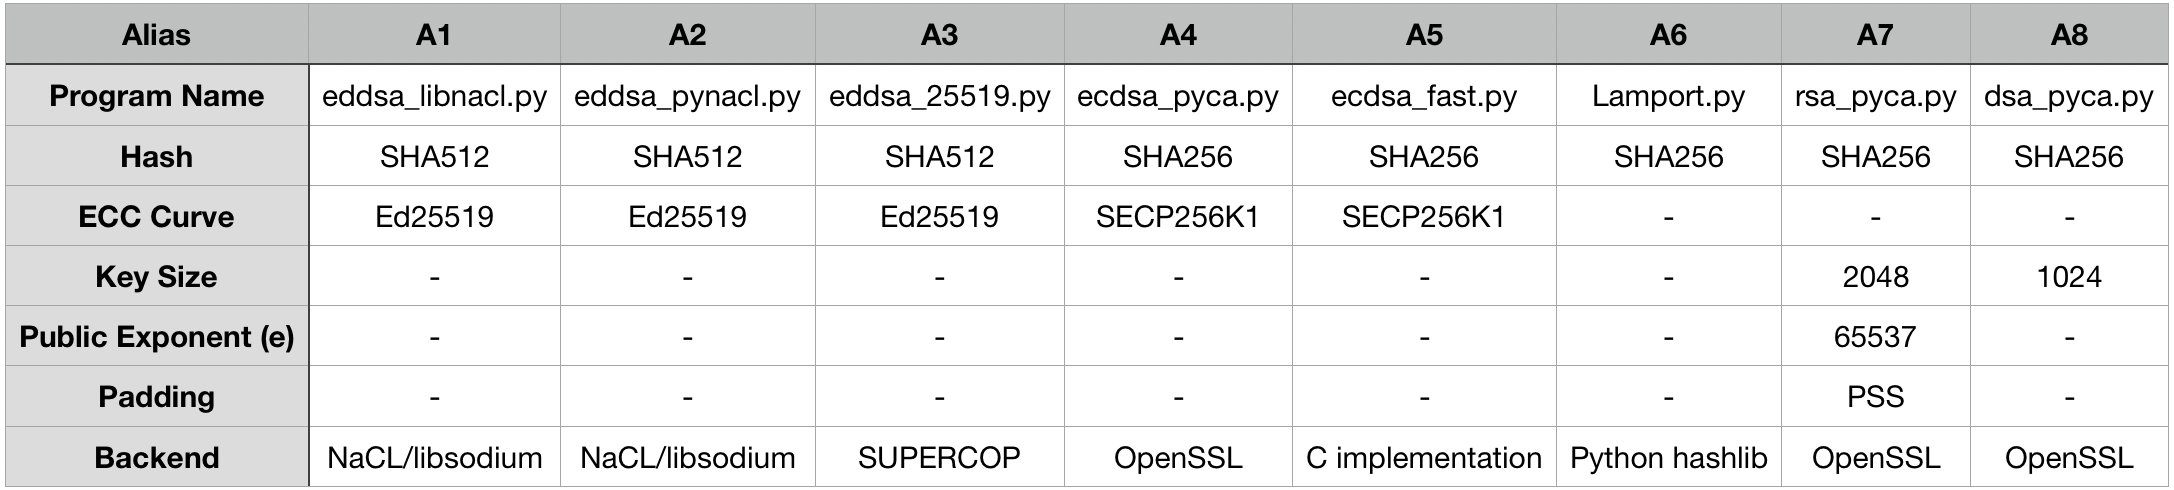
\includegraphics[scale=0.4]{Cross_Compare_Label.png}
\caption{\small{Cross Comparison Algorithms Setting and Parameter}}
\label{fig:Cross_Compare_Label}
\end{figure*}

\begin{figure*}
\centering
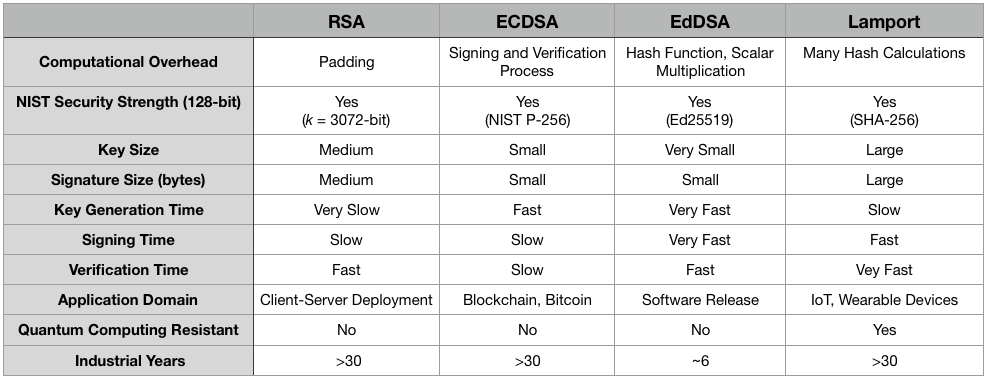
\includegraphics[scale=0.45]{Qualitative_Evaluation}
\caption{\small{Qualitative Evaluation of Digital Signature Schemes}}
\label{fig:Qualitative_Evaluation}
\end{figure*}

\section{Conclusion}

Table in Figure~\ref{fig:Qualitative_Evaluation} summarise the qualitative measures of our evaluation outcome among RSA, ECDSA, EdDSA and Lamport digital signature schemes. 

\noindent \textbf{Computational Overhead:} \quad In term of compute overhead, RSA has to consider padding and randomness scheme such as PSS. ECDSA inherits complex computation in its signing and verification process. EdDSA has to consider the built-in hash computation and its scalar multiplication. Lamport signature needs many hash calculations.

\noindent \textbf{Security Strength:} \quad In term of security strength, all algorithm can withstand NIST rating of security strength 128-bit \cite{nistKeysizes}, which is similar difficulty to breaking strong 128-bit block ciphers. With $2^{128}$ security target, RSA with key size 3072-bit, ECDSA with P-256, EdDSA with Ed25519 and Lamport signature with SHA-256 can achieve fairly strong security strength without compromising too much performance.

\noindent \textbf{Key Size:} \quad For the key size requirement, we rate RSA is medium, ECDSA key size is small, EdDSA key is the smallest and Lamport signature requires large key size.

\noindent \textbf{Signature Size:} \quad For the signature size in bytes comparison, RSA is medium, both ECDSA and EdDSA have comparatively smaller signature size than RSA, and Lamport signature is the largest. 

\noindent \textbf{Key Generation Time:} \quad In term of key generation time, RSA is the slowest, ECDSA is fast, EdDSA is the fastest and Lamport signature is slow. However, in real world RSA deployment, key generation is one-time effort as RSA key pair are re-used as long as private key is not compromised.

\noindent \textbf{Signing Time:} \quad For signing time, RSA and ECDSA are slow, Lamport is fast and EdDSA is the fastest.

\noindent \textbf{Verification Time:} \quad For signature verification, RSA and EdDSA are fast, ECDSA is slow and Lamport signature has the fastest verification time due to its solely use of hash values comparison.

\noindent \textbf{Quantum Computing Resistant:} \quad In term of future proof, only Lamport signature has the quantum-safe computing property due to its solely use of one-way hash property. Computational complexity based RSA and ECC algorithms are prone to Shor's algorithm \cite{Shor:1997:PAP:264393.264406} attack running on powerful quantum computing.

\noindent \textbf{Application Domain:} \quad In term of deployment, RSA is still dominant algorithm used in many Client-Server distributed systems such as certificate signing, secure-shell protocol, IPSecurity, so on. ECDSA is popular in blockchain technology and, especially employ in BitCoin (\url {https://bitcoin.org}) cryptocurrency. Lamport is popular in embedded and IoT device as well as when quantum proof classified secrecy is desired. EdDSA is popularly used in signing code and software releases and it has growing deployment as reported in \cite{ianix}. 

\noindent \textbf{Industrial Year:} \quad RSA, ECDSA and Lamport signature schemes have more than 30-years of industrial presence across many different type of deployment in applications and domains. Based on our experiment, EdDSA is the smallest and fastest digital signature scheme with comparable security strength to its counterpart. However, EdDSA is fairly new algorithm and, therefore, it has yet to be tested thoroughly to claim its superiority among digital signature schemes.

Based on the experiment presented, we conclude that our research contribute quantitative measurement and qualitative evaluation of the chosen digital signature schemes, observation over their characteristic and mathematical foundation and, critical analysis on three way implementation-performance-security trade-off and their applicable domains.

\subsection{Future Work}

For the future work, we would like to research more on definitive security evaluation of digital signature schemes. Power consumption observation is also another interesting evaluation metric to undertake experiment for deploying digital signature to ubiquitous mobile computing and IoT technology.


\subsection{Source Listing}

\begin{itemize}
    \item \url{https://github.com/victorskl/crypto-dsse}
    \item \url{https://github.com/victorskl/crypto-research-proposal}
    \item \url{https://github.com/victorskl/crypto-research-report}
    \item \url{https://youtu.be/jiIY31YrB-A}
\end{itemize}


\onecolumn

% \appendix
% \section{Appendix}

% 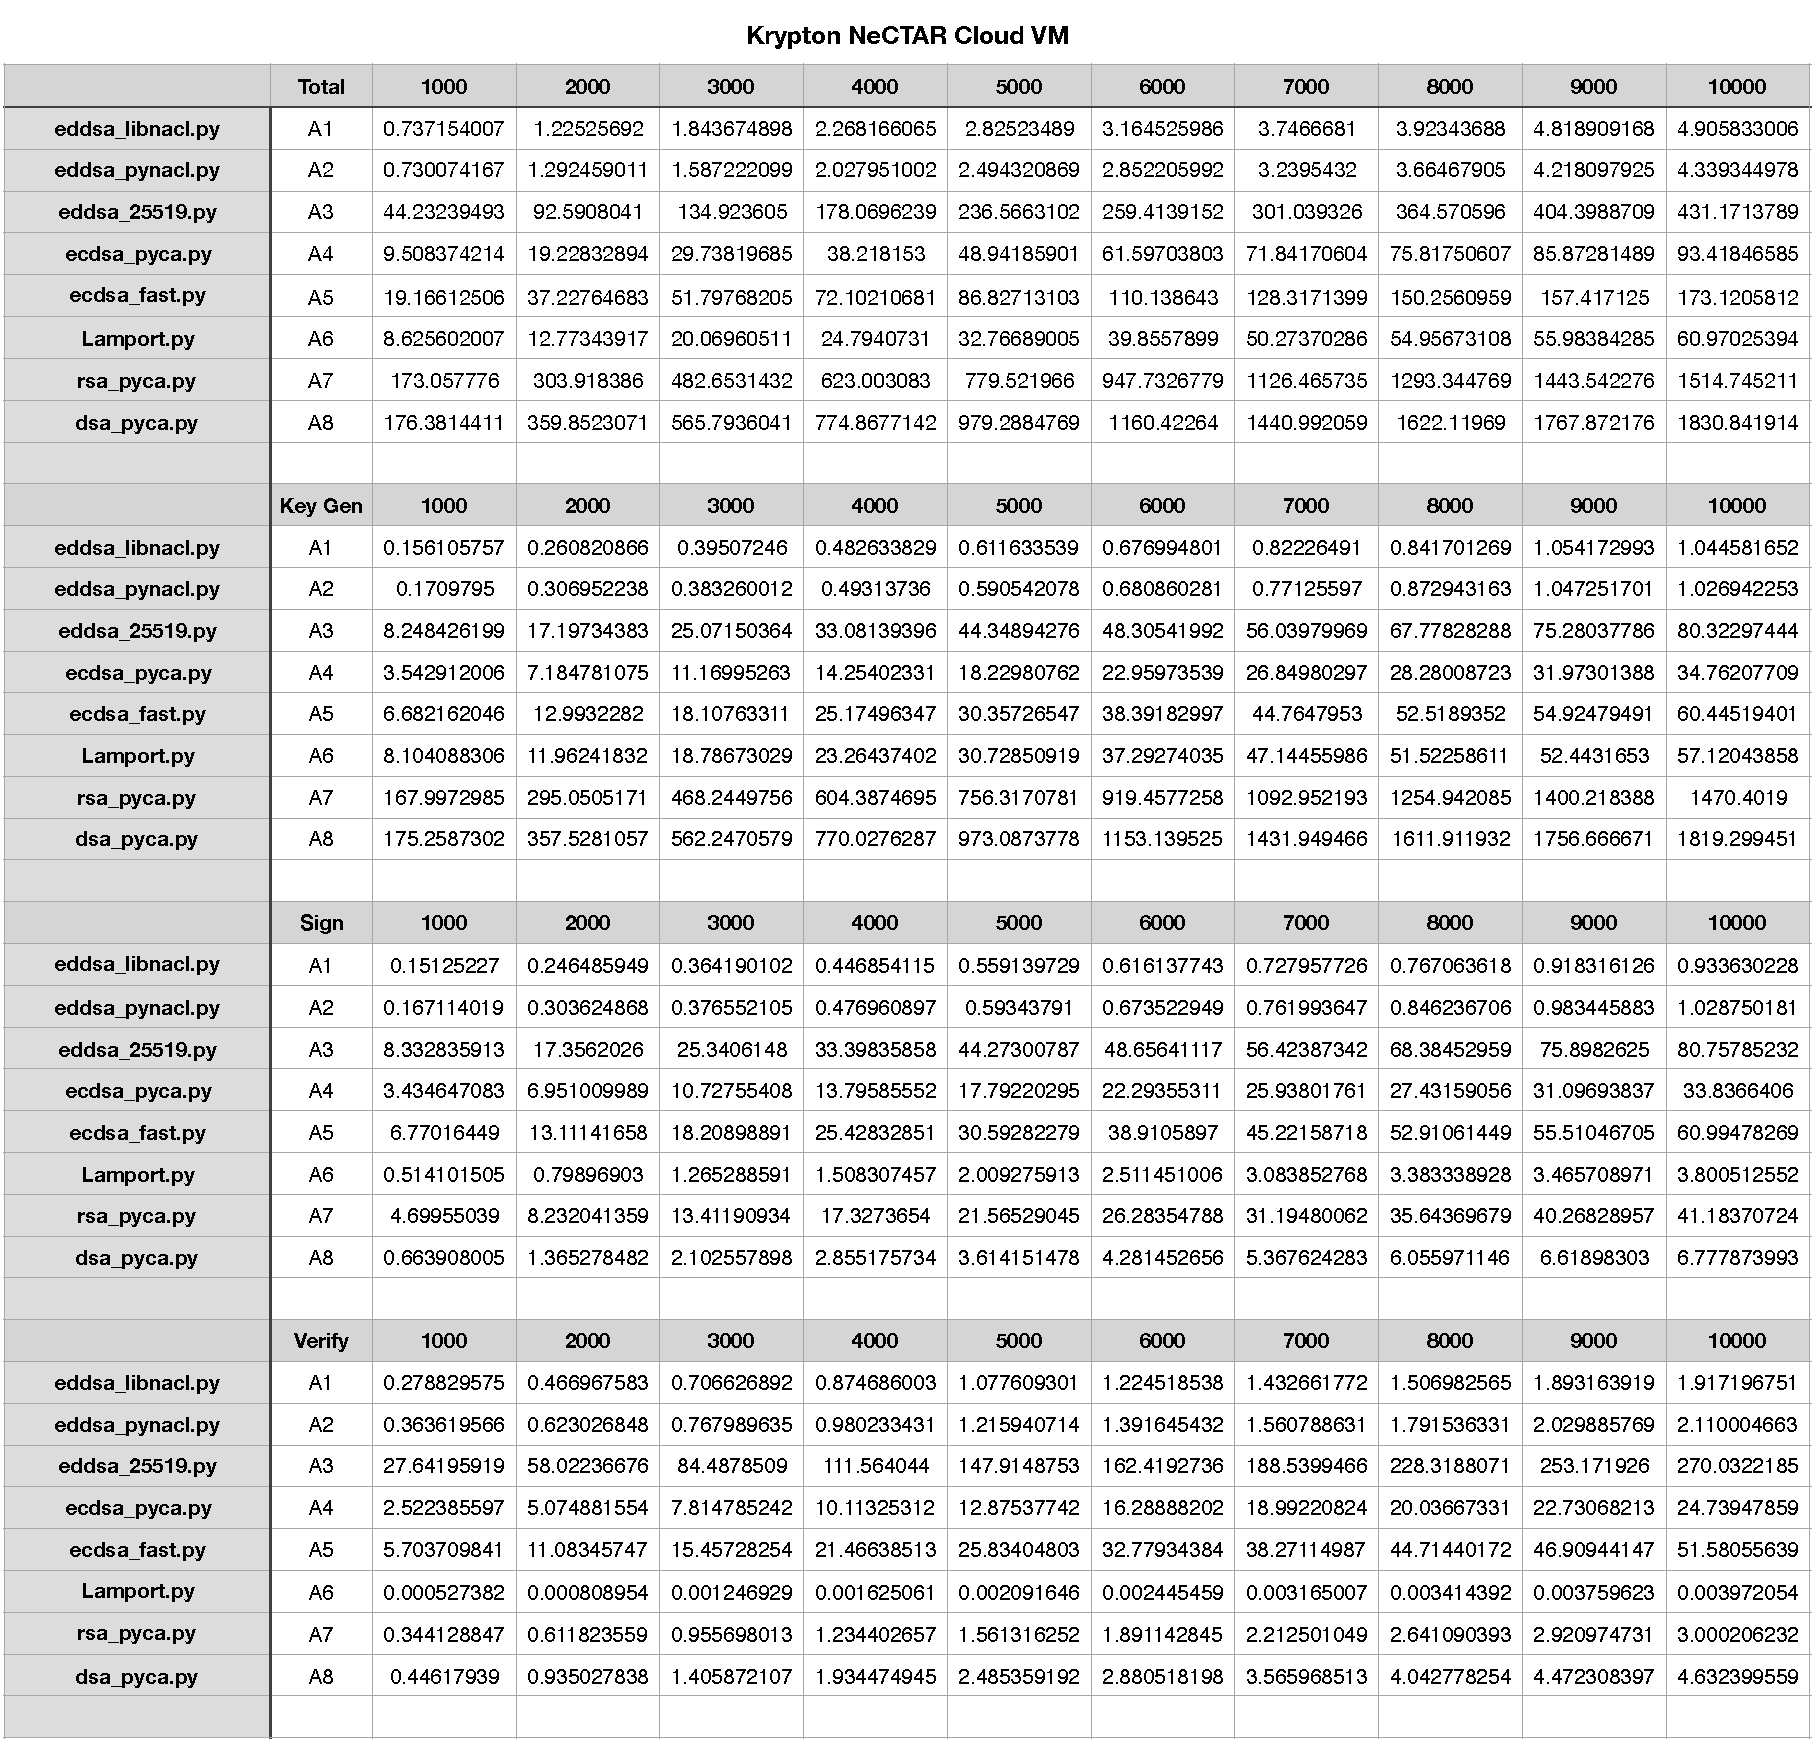
\includepdf[pages=-]{Cross_Compare_Krypton_Runtimes.pdf}
% 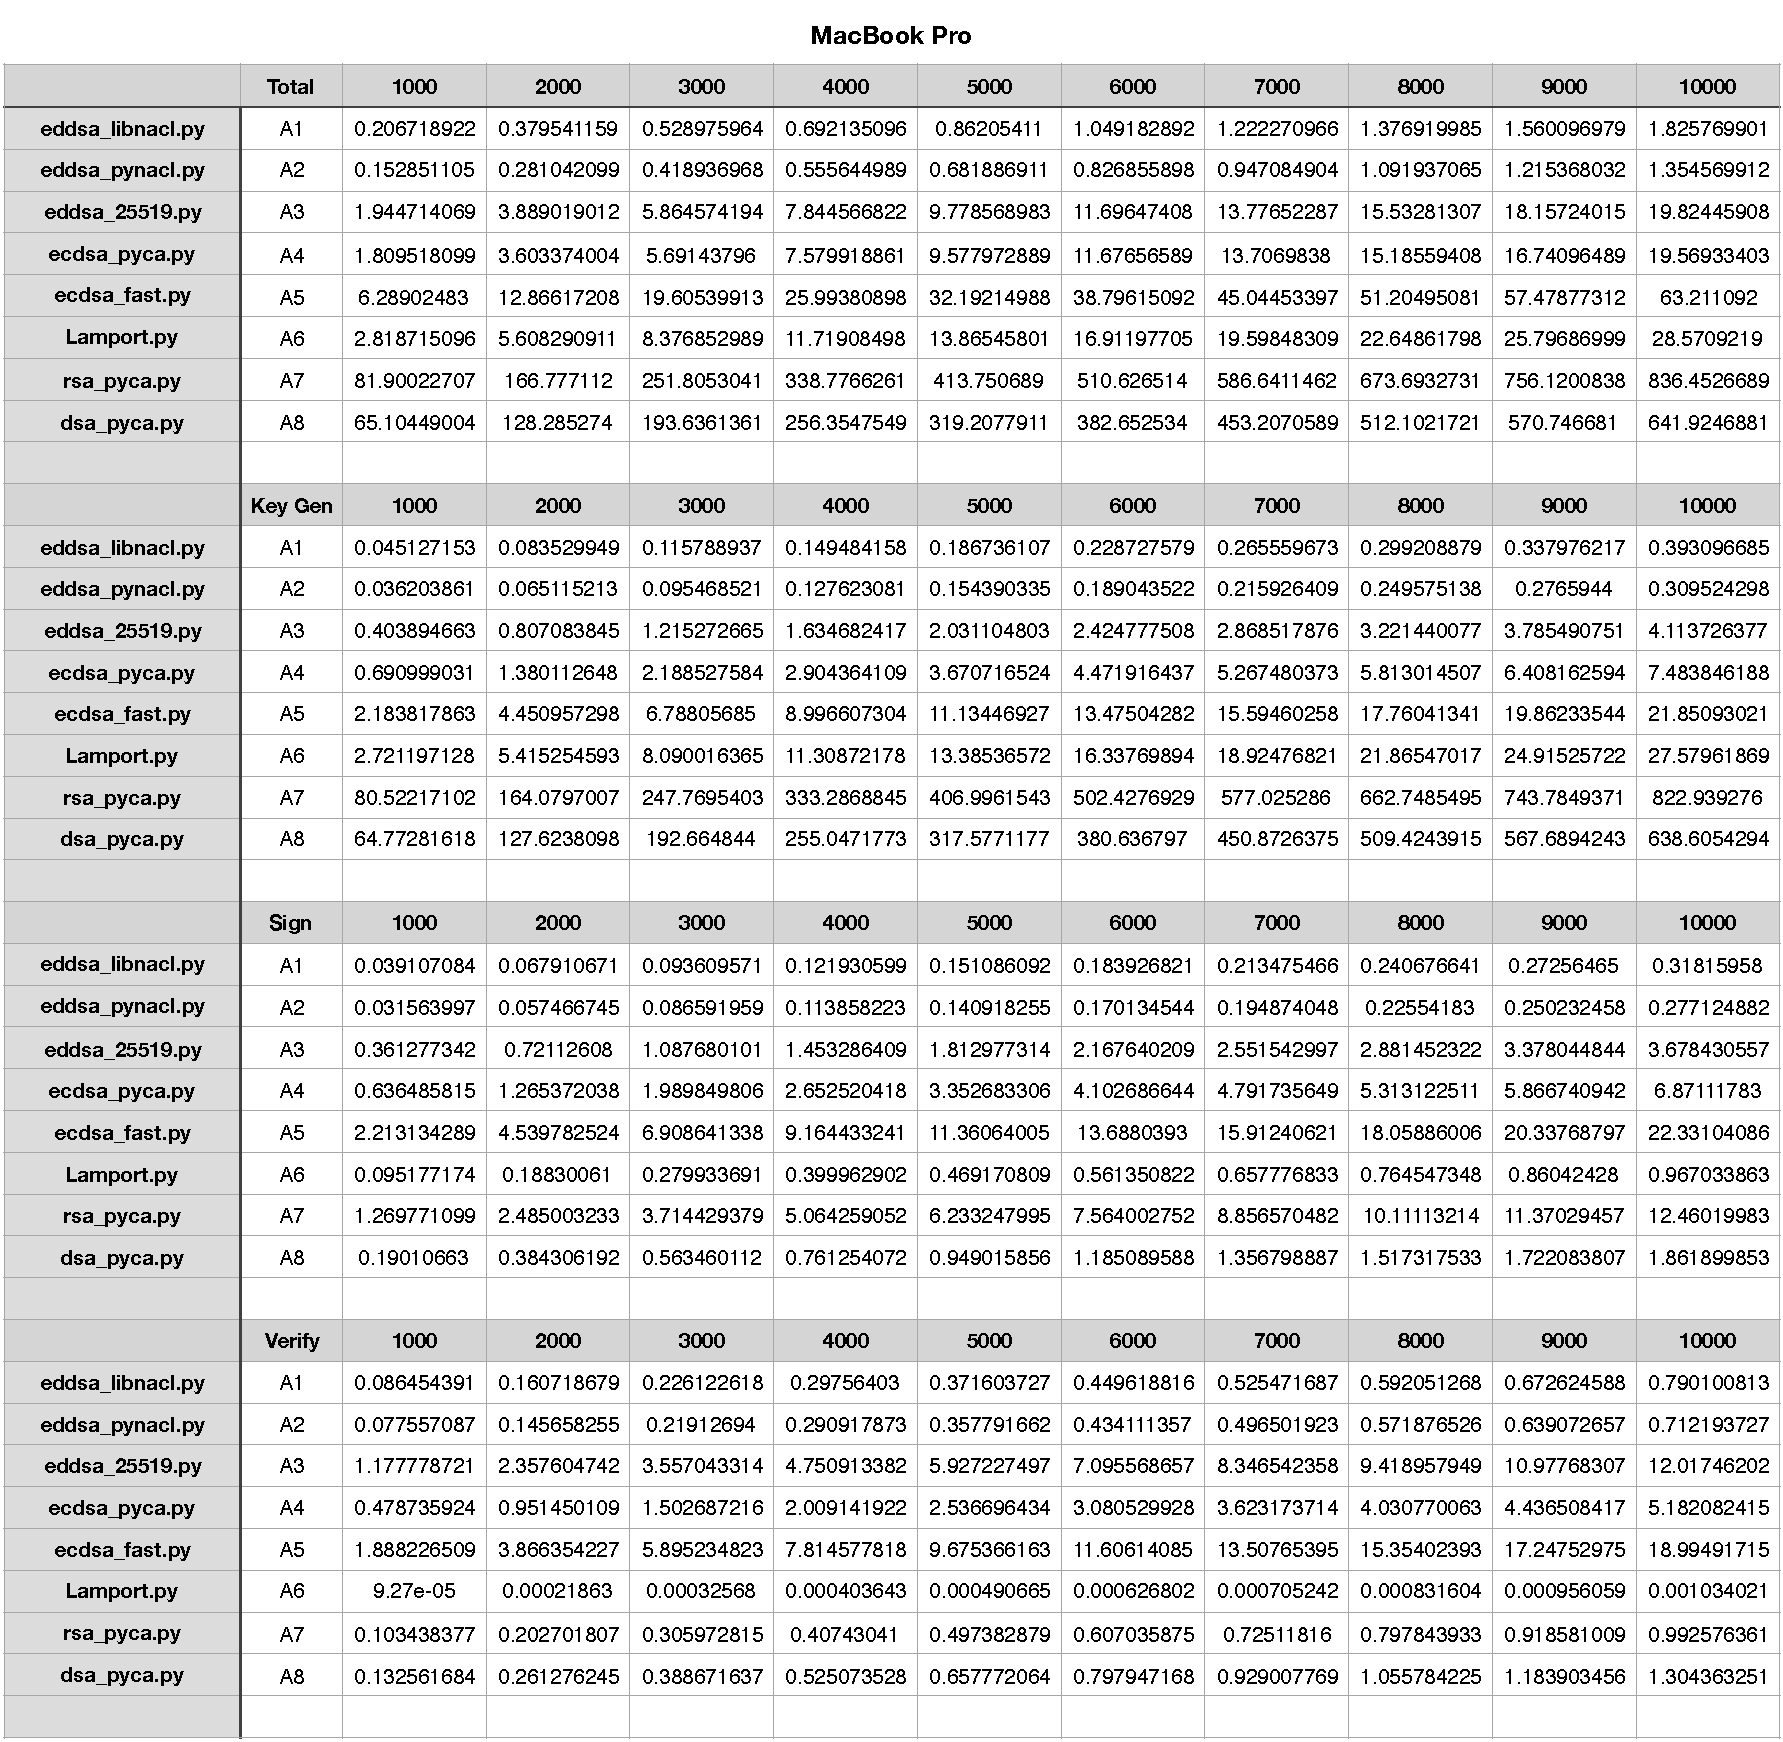
\includepdf[pages=-]{Cross_Compare_MacBookPro_Runtimes.pdf}

\begin{figure}
\centering
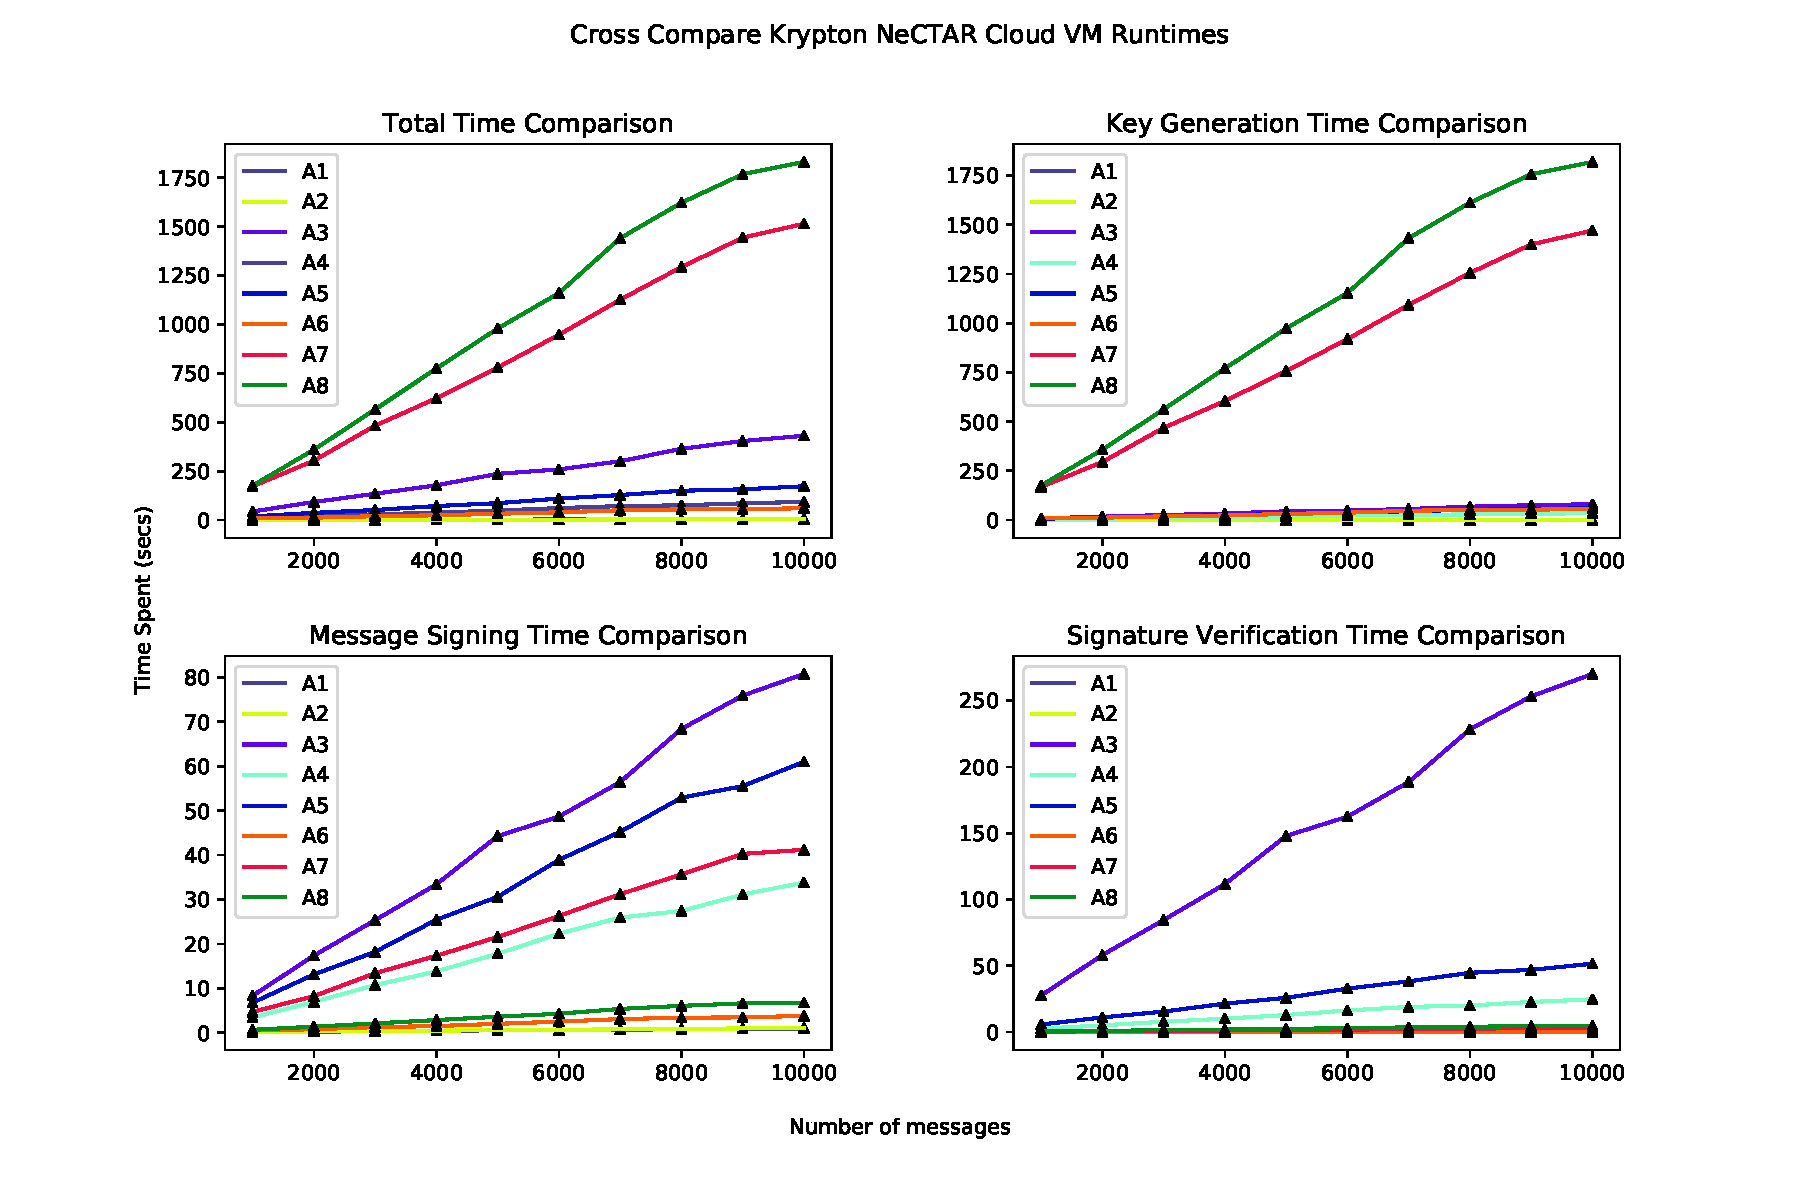
\includegraphics[scale=0.6]{Cross_Compare_Krypton_Runtimes_Graph}
\caption{\small{Cross Compare Krypton NeCTAR Cloud VM Runtimes}}
\label{fig:Cross_Compare_Krypton_Runtimes_Graph}
\end{figure}

\begin{figure}
\centering
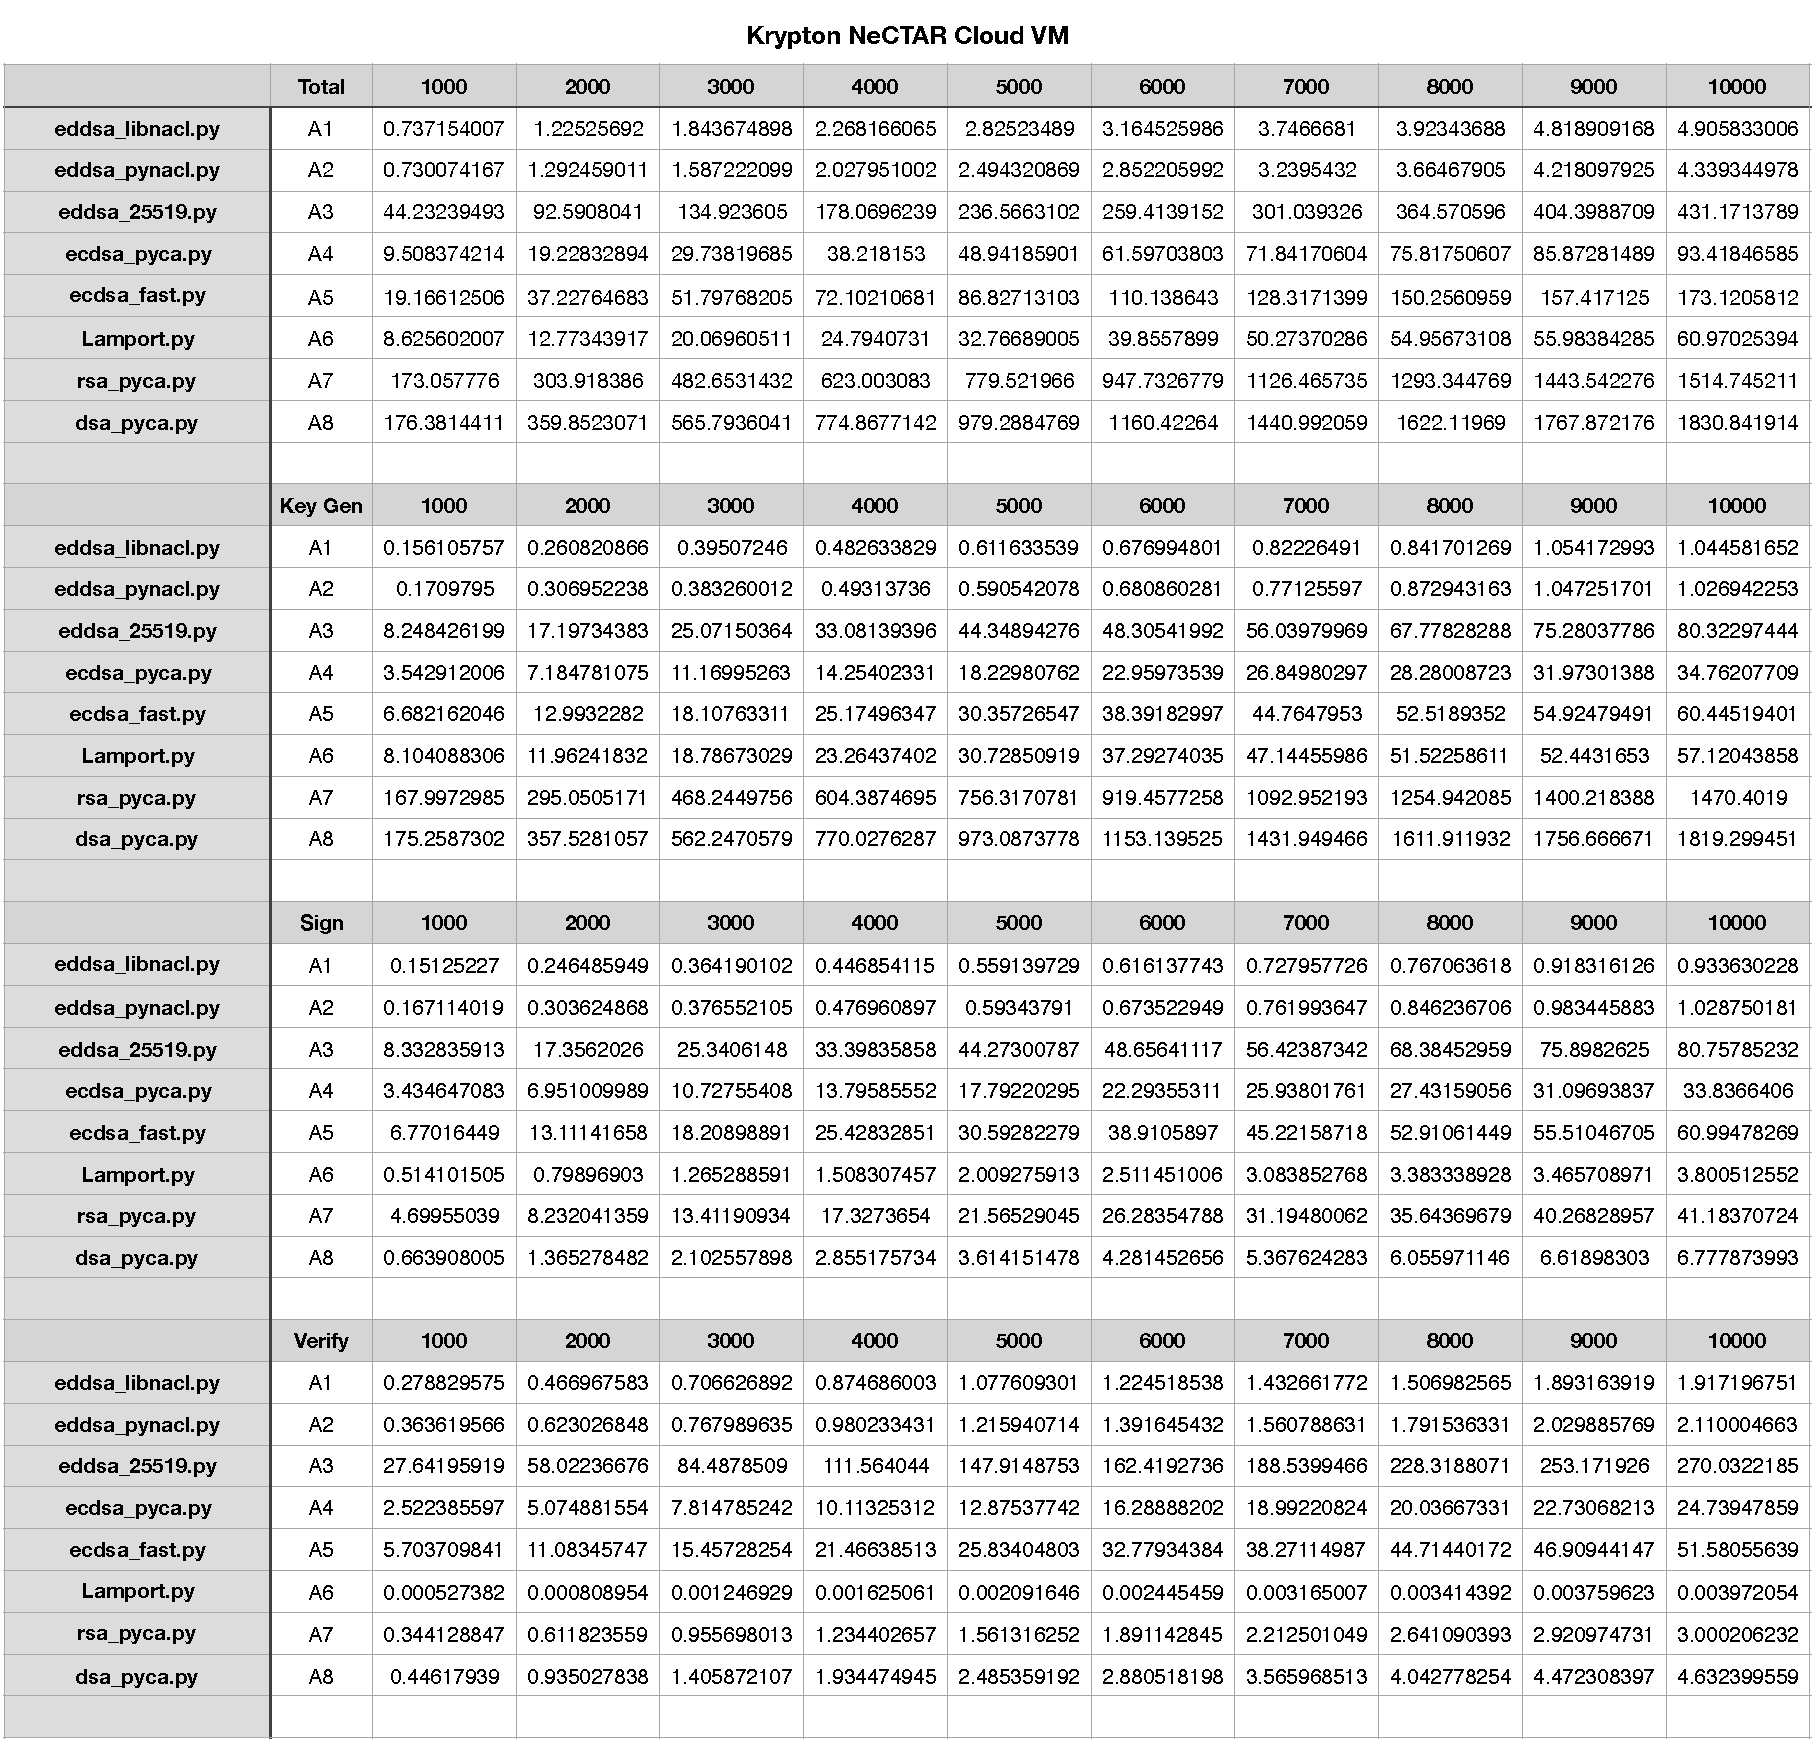
\includegraphics[scale=0.5]{Cross_Compare_Krypton_Runtimes}
\caption{\small{Cross Compare Krypton NeCTAR Cloud VM Runtimes Table}}
\label{fig:Cross_Compare_Krypton_Runtimes}
\end{figure}

\begin{figure}
\centering
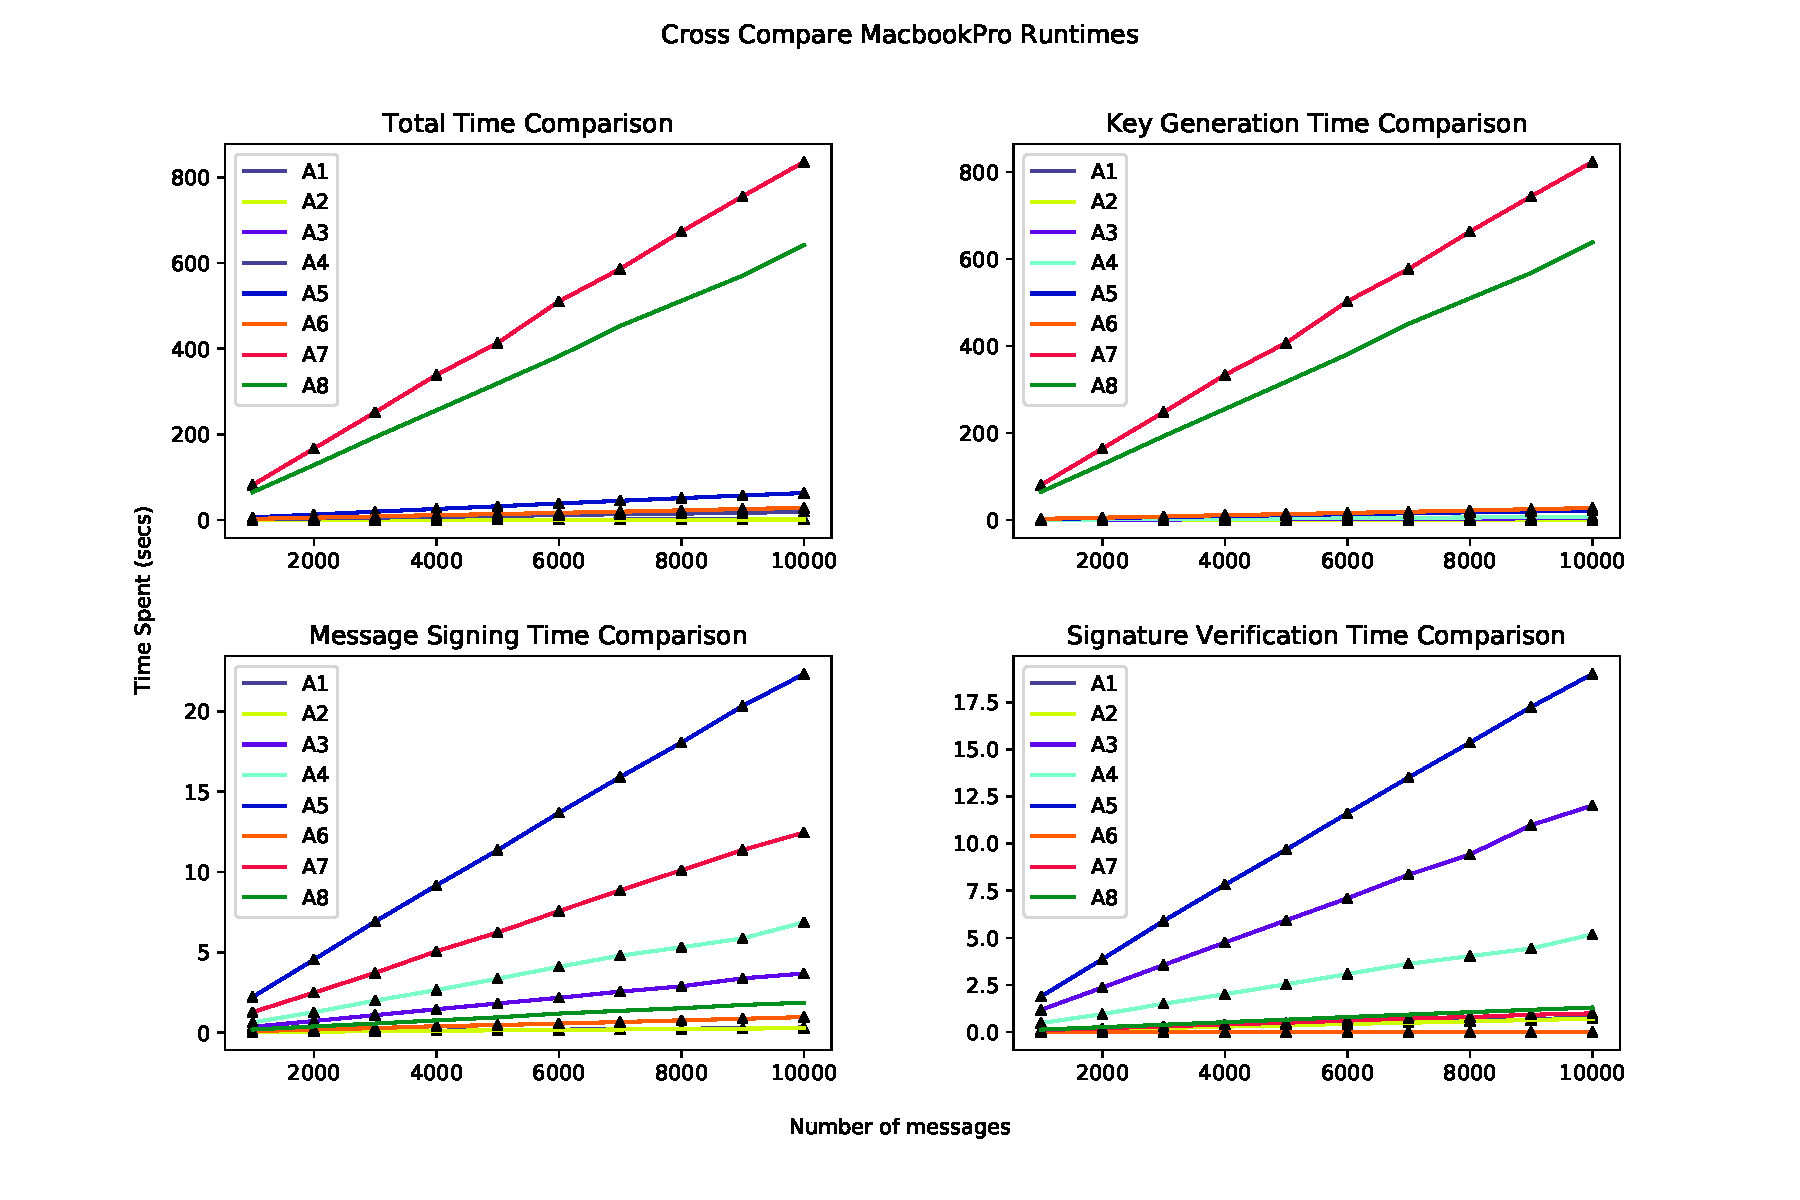
\includegraphics[scale=0.6]{Cross_Compare_MacBookPro_Runtimes_Graph}
\caption{\small{Cross Compare MacBookPro Runtimes}}
\label{fig:Cross_Compare_MacBookPro_Runtimes_Graph}
\end{figure}

\begin{figure}
\centering
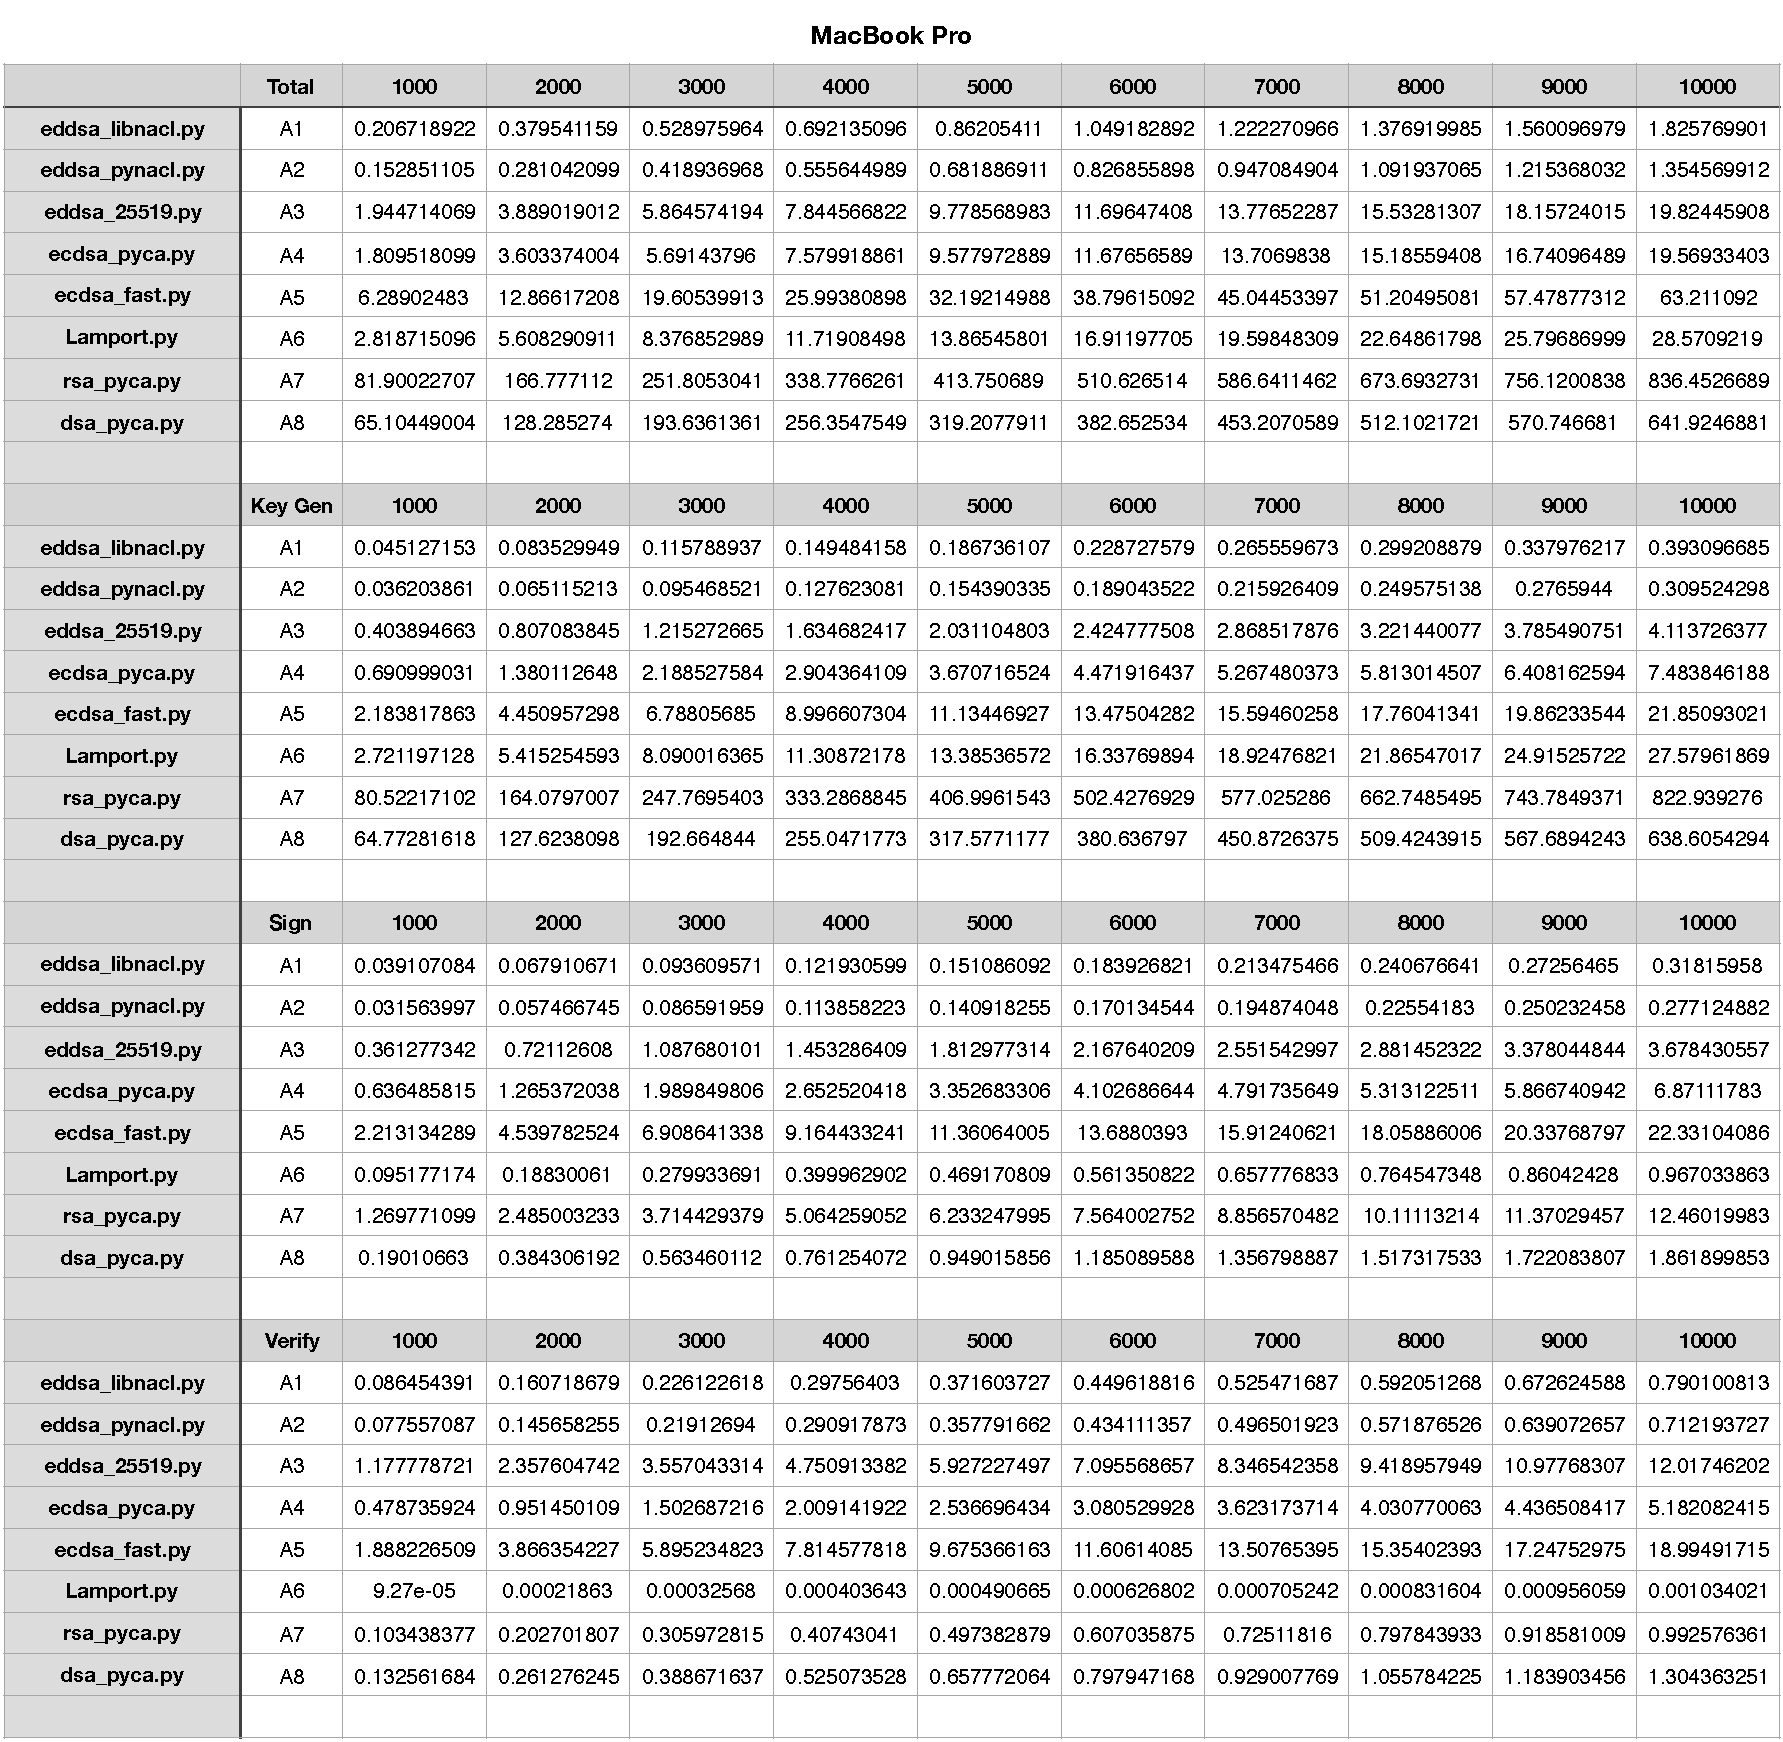
\includegraphics[scale=0.5]{Cross_Compare_MacBookPro_Runtimes}
\caption{\small{Cross Compare MacBookPro Runtimes Table}}
\label{fig:Cross_Compare_MacBookPro_Runtimes}
\end{figure}

\twocolumn

\bibliographystyle{unsrt}
\bibliography{references}


\end{document}
